%%
%% Copyright 2022 OXFORD UNIVERSITY PRESS
%%
%% This file is part of the 'oup-authoring-template Bundle'.
%% ---------------------------------------------
%%
%% It may be distributed under the conditions of the LaTeX Project Public
%% License, either version 1.2 of this license or (at your option) any
%% later version.  The latest version of this license is in
%%    http://www.latex-project.org/lppl.txt
%% and version 1.2 or later is part of all distributions of LaTeX
%% version 1999/12/01 or later.
%%
%% The list of all files belonging to the 'oup-authoring-template Bundle' is
%% given in the file `manifest.txt'.
%%
%% Template article for OXFORD UNIVERSITY PRESS's document class `oup-authoring-template'
%% with bibliographic references
%%
%%%%%%% To do
% 1. Change mapping to mapping. species mapping,
%    reaction mapping, (structural) mapping: relates reference to target via reaction and species mapping to find a subnet of the target that is structurally identical to the reference
% 2. Put BioModels analysis in discussion? Eliminate parallel processing discussion?

%%%CONTEMPORARY%%%
% do not want numbering, add 'unnumsec' in the bracket
%\documentclass[webpdf,contemporary,large, draft]{oup-authoring-template}
\documentclass[webpdf,contemporary,large]{oup-authoring-template}


%\onecolumn % for one column layouts

%\usepackage{showframe}

\graphicspath{{Fig/}}

% new commands
\newcommand{\revision}[1]{\color{red}{#1 }\color{black}}
\newcommand{\revisionb}[1]{\color{red}{#1}\color{black}}
\newcommand{\comment}[2]{
  \color{red} *{#1}*{\bf #2} \color{black}}
\newcommand{\question}[2]{
  \color{green} *{#1}*{#2} \color{black}}
\newcommand{\reply}[2]{
  \color{brown} *{#1}*{#2} \color{black}}
\newcommand\note[1]{\textcolor{blue}{#1}}

% referencing figures and tables and equations
\newcommand{\eqnref}[1]{
  Eq.~\ref{#1}}
\newcommand{\fig}[1]{
  Fig.~\ref{#1}}
\newcommand{\tab}[1]{
  Tab.~\ref{#1}}
\newcommand{\secref}[1]{Section~\ref{#1}}
% Macros
\newcommand{\mat}[1]{${\bf #1}$} % version 1
\newcommand{\net}[1]{$\mathcal{N}_#1$} % version 1
\newcommand{\rnet}{$\mathcal{R}$} % version 1
\newcommand{\tnet}{$\mathcal{T}$} % version 1
\newcommand{\cmat}[1]{${\bf #1}^{\bf c}$} % version 1
\newcommand{\ctwomat}[1]{${\bf #1}^{{\bf c}^2}$} % version 1
\newcommand{\crow}[2]{${\bf #1}^{\bf c}_{#2 \star}$}  % compat mat row
\newcommand{\ccol}[2]{${\bf #1}^{\bf c}_{\star #2$}} % compat mat col
\newcommand{\mcol}[2]{${\bf #1}_{\star #2}$}  % mat row
\newcommand{\mrow}[2]{${\bf #1}_{#2 \star}$}  % mat col
\newcommand{\col}[1]{$_{\star #1}$}
\newcommand{\Kappa}{\mathrm{K}}
\newcommand{\py}{\texttt{pySubnetSB}}

% Package used  
\usepackage{adjustbox}
\usepackage{listings}
\usepackage{color}    
\usepackage{amsmath}
\usepackage{amssymb}
\usepackage{framed}
\usepackage{natbib}
\setcitestyle{square, comma, citesep={\,;}, numbers, sort&compress}
\usepackage{graphicx}
\usepackage{hyperref}
\usepackage{fancyvrb}
\usepackage{xcolor}
\hypersetup{
    colorlinks,
    linkcolor={red!50!black},
    citecolor={blue!50!black},
    urlcolor={blue!80!black}
}

\usepackage{natbib}
\setcitestyle{square, comma, citesep={\,;}, numbers, sort&compress}

\theoremstyle{thmstyleone}%
\newtheorem{theorem}{Theorem}%  meant for continuous numbers
% \newtheorem{theorem}{Theorem}[section]
% meant for sectionwise numbers
%% optional argument [theorem] produces theorem numbering sequence instead of independent numbers for Proposition
\newtheorem{proposition}[theorem]{Proposition}%
%%\newtheorem{proposition}{Proposition}% to get separate numbers for theorem and proposition etc.
\theoremstyle{thmstyletwo}%
\newtheorem{example}{Example}%
\newtheorem{remark}{Remark}%
\theoremstyle{thmstylethree}%
\newtheorem{definition}{Definition}

\begin{document}

\journaltitle{Bioinformatics}
\DOI{DOI HERE}
\copyrightyear{2025}
\pubyear{2025}
%\access{Advance Access Publication Date: Day Month Year}
\appnotes{Paper}

\firstpage{1}

\title[]{Discovering Subnetworks in SBML Models}

\author[1,2,3]{Joseph L. Hellerstein}
\author[2]{Lucian P. Smith}
\author[4]{Lillian T. Tatka}
\author[3]{Steven S. Andrews}
\author[5]{Michael A. Kochen}
\author[1,3]{Herbert M. Sauro}

\address[1]{
  \orgdiv{eScience Institute},
  \orgname{University of Washington},
  \orgaddress{Seattle, WA},
  \country{USA}
}
\address[2]{
  \orgdiv{Paul G. Allen School of Computer Science},
  \orgname{University of Washington},
  \orgaddress{Seattle, WA},
  \country{USA}
}

\address[3]{
\orgdiv{Department of Bioengineering}, 
\orgname{University of Washington},
\orgaddress{Seattle, WA},
\country{USA}
}

\address[4]{
\orgdiv{Talus Bioscience},
\orgaddress{Seattle, WA},
\country{USA}
}
\address[5]{
\orgdiv{Software Applications and Technology, Rocky Mountain Division},
\orgname{Applied Research Associates, Inc.},
\orgaddress{Bentonville AR},
\country{USA}
}


\corresp{$^\ast$Corresponding author: Joseph L Hellerstein, jlheller@uw.edu}


\received{Date}{0}{Year}
\revised{Date}{0}{Year}
\accepted{Date}{0}{Year}


\abstract{{\bf Motivation:} Many advances in biomedical research are driven by structural analysis, which investigates
interconnections between elements in biological systems (e.g. structural analysis of proteins to infer their function).
Herein, we consider
{\bf subnet discovery} in chemical reaction networks (CRNs)--discovering a subset of a target CRN that is
structurally identical to a reference CRN.
Structural analysis techniques such as
motif finding and graph mining look for small, arbitrary, and commonly occurring substructures (e.g. 3 gene feedforward loops).
In contrast,
subnet discovery looks for larger, specific, and infrequently occurring substructures (e.g. 10 reaction mitogen-activated protein kinase (MAPK) pathway).
%Applications of subnet discovery include the discovery of conserved chemical pathways and the elucidation of the structure of complex CRNs.
Subnet discovery is an NP-hard subgraph problem.
We are unaware of existing tools for subnet discovery in CRNs.
%This is in large part due to the special characteristics of CRN graphs, that they are directed, bipartite, hypergraphs.
\newline
{\bf Results:} We introduce \py{}, an open source Python package for discovering subnets in CRNs that are represented in the Systems Biology Markup Language (SBML) community standard. 
%\py{} employs a constraint-based approach that  greatly reduces computations for subnet discovery.
\revision{We show that
\py{} achieves large reductions in computational complexity for subnet discovery. For example, in studies of randomly selected target networks
with 100 reactions each with a random reference network with 20 reactions, computations are reduced from an infeasible $10^{78}$ evaluations to a more practical $10^{8}$ evaluations.}
%, and
%Furthermore, our implementation 
%provides 
%large speedups for subnet evaluations.
We develop a methodology for assessing the statistical significance of subnet discovery.
Last, we study subnets in BioModels
for approximately 200,000 pairs of reference and target models.
We show that for a reference MAPK pathway, subnet discovery correctly indicates the presence of MAPK function in several target models.
The studies also suggest two interesting hypotheses: (a) the potential presence of hidden oscillators in several models in BioModels,
and (b) the possibility of a conserved mechanism for intracellular immune response.
\newline
\textbf{Availability:} \py{} is installed using {\tt pip install pySubnetSB}, and is hosted at \url{https://github.com/ModelEngineering/pySubnetSB/}.
%\url{https://github.com/ModelEngineering/pySubnetSB/blob/main/examples/api_basics.ipynb} is a Jupyter notebook that demonstrates \texttt{pySubnetSB} capabilities.\\
\textbf{Contact:} \href{jlheller@uw.edu}{jlheller@uw.edu}  
}
%\textbf{Supplementary information:} 

\keywords{systems biology, model development, SBML, model, subgraph problem}

\maketitle

\section{Introduction}

%%%%%%%%FIGURE%%%%%%%%%%%%%%%%
\begin{figure}%
\centering
\begin{minipage}{1.3in}
{\tiny
\begin{verbatim}
J1: -> BCG
J2:  -> Effector_cells
J3: Effector_cells ->
J4: -> Tumor_uninfected_cells
J5: BCG + Tumor_uninfected_cells 
   -> Tumor_infected_cells
J6: Tumor_infected_cells ->
J7: BCG ->
\end{verbatim}
\vspace{0.38in}
{\bf (a) Model 1034}
}
\end{minipage}
\qquad
\begin{minipage}{1.3in}%
{\tiny
\begin{verbatim}
v01: A + I -> D_IA
v02: I + I -> D_II
v03: I ->
v04: A ->
v05: D_IA ->
v06: D_II ->
v07: D_IA -> A
v08: D_II -> I
v09: R ->
v10: -> I
v11: -> A
v12: -> R 
\end{verbatim}
{\bf (b) Model 351}
}
\end{minipage}%
\caption{Two models in BioModels. The running example uses Model 1034 as the reference network and Model 351 as the target network.}
\label{fig:running-example-models}
\end{figure}
%%%%%%%%END FIGURE%%%%%%%%%%%%%%%%                                                                                                                
\begin{figure}
%\centering
%\begin{subfigure}{0.7\textwidth}
%{\tiny
%\begin{tabular}{|l||c|c|c|c|c|c|c|}
%\hline
%{\bf species} & {\bf J1} & {\bf J2} & {\bf J3} & {\bf J4} & {\bf J5} & {\bf J6} & {\bf J7} \\
%\hline\hline
%BCG & 0 & 0 & 0 & 0 & 1 & 0 & 1\\
%Effector\_cells & 0 & 0 & 1 & 0 & 0 & 0 & 0\\
%Tumor\_uninfected\_cells & 0 & 0 & 0 & 0 & 1 & 0 & 0\\
%Tumor\_infected\_cells & 0 & 0 & 0 & 0 & 0 & 1 & 0\\
%\hline
%\end{tabular}
%}
%    \caption{Reaction Stoichiometry}
%    \label{fig:biomodels1034}
%\end{subfigure}
%%%
%\begin{subfigure}{0.7\textwidth}
%\vspace{10pt}
%{\tiny
%\begin{tabular}{|l||c|c|c|c|c|c|c|}
%\hline
%{\bf species} & {\bf J1} & {\bf J2} & {\bf J3} & {\bf J4} & {\bf J5} & {\bf J6} & {\bf J7} \\
%\hline\hline
%BCG & 1 & 0 & 0 & 0 & 0 & 0 & 0\\
%Effector\_cells & 0 & 1 & 0 & 0 & 0 & 0 & 0\\
%Tumor\_uninfected\_cells & 0 & 0 & 0 & 1 & 0 & 0 & 0\\
%Tumor\_infected\_cells & 0 & 0 & 0 & 0 & 1 & 0 & 0\\
%\hline
%\end{tabular}
%}
% \caption{Product Stoichiometry}
%\end{subfigure}
%%%
%\begin{subfigure}{0.7\textwidth}
%\vspace{10pt}
%{\tiny
%\begin{tabular}{|l||c|c|c|c|c|c|c|}
%\hline
%{\bf species} & {\bf J1} & {\bf J2} & {\bf J3} & {\bf J4} & {\bf J5} & {\bf J6} & {\bf J7} \\
%\hline\hline
%BCG & 1 & 0 & 0 & 0 & 0 & 0 & -1\\
%Effector\_cells & 0 & 1 & -1 & 0 & 0 & 0 & 0\\
%Tumor\_uninfected\_cells & 0 & 0 & 0 & 1 & -1 & 0 & 0\\
%Tumor\_infected\_cells & 0 & 0 & 0 & 0 & 1 & -1 & 0\\
%\hline
%\end{tabular}
%}
% \caption{Standard Stoichiometry}
%\end{subfigure}
%%%
%\caption{Stoichiometry matrices for BioModels 1034.}
%\label{fig:running-example-models}
%\end{figure}
%%%%%%%%%FIGURE%%%%%%%%%%%%%%%%       

%%%%%%%%FIGURE%%%%%%%%%%%%%%%%
%\begin{figure}
%\centering                                                                                                                                                 
%\begin{minipage}{1.2in}
%{\tiny
%\begin{tabular}{|l|l|} 
%\hline
%1034 & 351 \\
%\hline\hline
%BCG & I \\  
%Effector\_cells & R \\
%Tumor\_uninfected\_cell & A \\
%Tumor\_infected\_cell & D\_IA \\
%\hline
%\end{tabular}
%
%\vspace{0.4in}
%{\bf (a) species mapping}
%}
%\end{minipage}
%%%
%\qquad
%\begin{minipage}{0.7in}%
%{\tiny
%\begin{tabular}{|c|c|} 
%\hline
%1034 & 351 \\
%\hline\hline
%J1 & v10 \\  
%J2 & v12 \\
%J3 & v09 \\
%J4 & v11 \\
%J5 & v01 \\
%J6 & v05 \\
%J7 & v03 \\
%\hline
%\end{tabular}
%
%\vspace{0.1in}
%{\bf (b) reaction mapping}
%}
%\end{minipage}  
%%%
%\qquad
%\begin{minipage}{0.4in}%
%{\tiny
%\begin{verbatim}
%v10:  -> I
%v12:  -> R
%v09: R -> 
%v11:  -> A
%v01: A + I -> D_IA
%v05: D_IA -> 
%v03: I -> 
%\end{verbatim}
%\vspace{0.15in}
%{\bf (c) inferred network}
%}
%\end{minipage}
%\hfill                
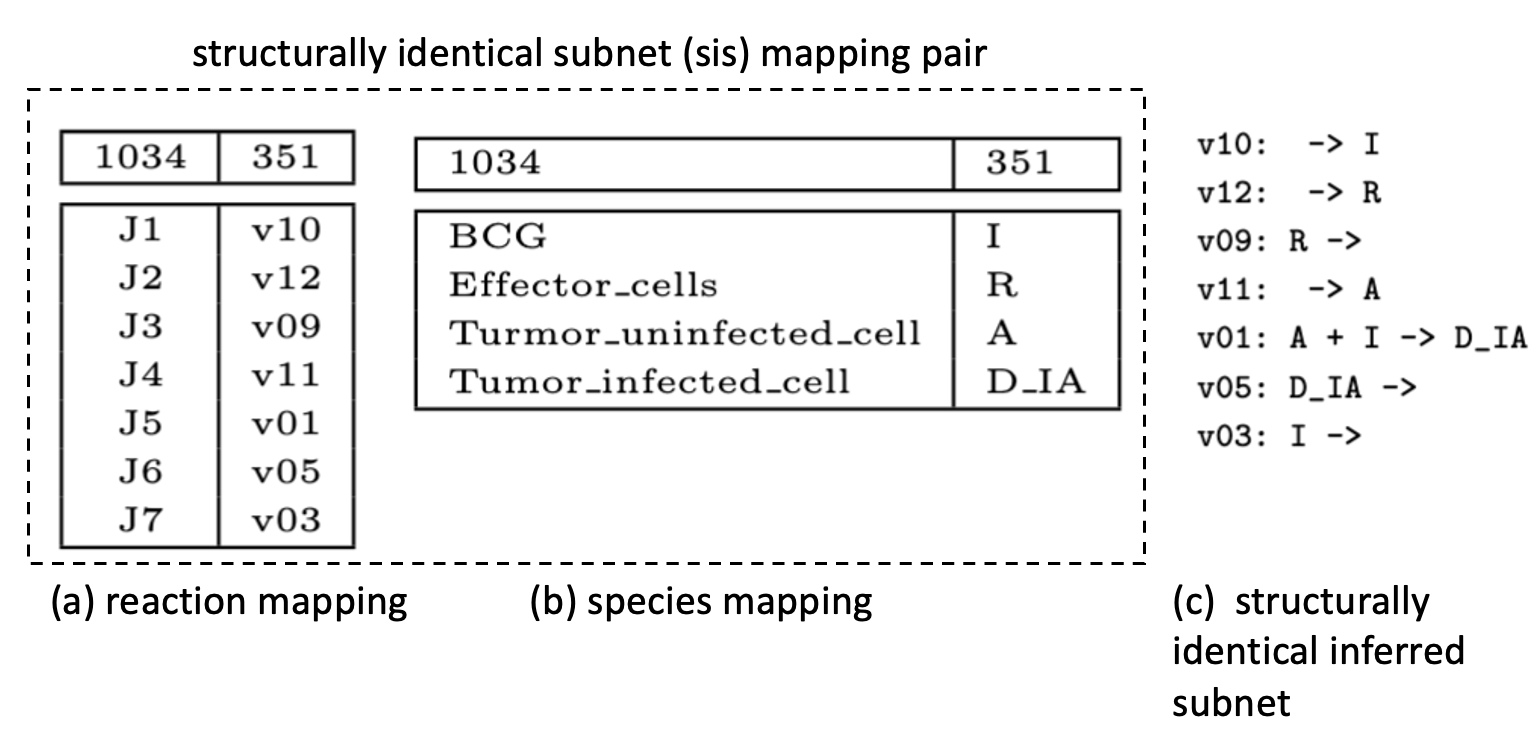
\includegraphics[width=0.5\textwidth, angle=0]{figures/example-mapping.png}
%%
\caption{Mapping pairs and inferred subnet. The \revision{reation} mapping in (a) in combination with the \revision{species} mapping in (b) is a mapping pair that identifies the inferred subnet of Model 351 in (c) that is is structurally identical to Model \revisionb{1034}.}
\label{fig:running-example-induced-network}
\end{figure}
%%%%%%%%FIGURE%%%%%%%%%%%%%%%%
Many insights in biomedical research are driven by structural analysis, which investigates
the interconnections between elements in biological systems.
Examples include:
structural analysis of proteins to infer their function (e.g. \citep{osadchy_maps_2011}); analyzing chemical pathways to identify drug targets (e.g. \citep{paul_artificial_2021});
%molecular evolution and phylogenetics (e.g. \citep{10.1093/oso/9780195135848.001.0001});
structures in chemical reaction networks related to functions such as signal amplification and error detection \citep{hartwell_molecular_1999};
%achieving robustness through the structure of metabolic networks (e.g. ref?? Stelling, Palsson);
and the function of gene motifs in gene regulatory networks (e.g. \citep{Alon2007}).
Structural analysis is often successful because: (a) structural information is much easier to obtain and generally more accurate than dynamics such as species concentrations and reaction fluxes; and (b)
biological structures can be closely related to their function (e.g. \citep{sharan_modeling_2006}).
Many tools have been developed for analyzing biological structures, such as:
Basic Local Assignment Search Tool (BLAST) for sequences \citep{mcginnis_blast_2004}; graph mining to discover frequently occurring substructures \citep{lambusch_identifying_2018}; and developing signatures for substructures related to their biological function \citep{shellman_network_2013}.

Our focus is on {\bf chemical reaction networks (CRNs)} in biological systems.
In particular, we develop a tool for discovering subnetworks (hereafter just subnets) in CRNs.
By {\bf subnet discovery}, we mean determining if a {\bf reference CRN} is structurally identical to a subnet of a {\bf target CRN} in that there is an equivalence between the reference reactions and chemical species and the reactions and species in a subnet of the target.

At first glance, subnet discovery seems to overlap with motif finding and graph mining, techniques that look for small, arbitrary, and commonly occurring substructures (e.g. 3 gene feedforward loops \citep{Alon2007}).
In contrast,
subnet discovery looks for larger, more specific, and infrequently occurring substructures.
For example, \secref{sec:biomodels} discusses subnet discovery using the mitogen-activated protein kinase (MAPK) pathway, a specific 10 reaction system that occurs only once in each of its targets.

We believe that subnet discovery is of particular interest for the following use cases.
\begin{itemize}
\item {\bf Use case 1: Infer function in the target from the reference.}
If a reference CRN is a subnet of a target CRN, then 
the functions provided by the reference (e.g. oscillation) {\em might} be present in the target.
\item {\bf Use case 2: Infer conserved mechanisms in targets that have the same reference.}
If many target CRNs
have the same reference as a subnet, then the reference {\em might} implement mechanisms that are conserved in the targets.
\end{itemize}
\secref{sec:biomodels} provides examples of both use cases.
We emphasize that like motif finding and graph mining, the objective of subnet discovery is to identify interesting hypotheses.
In general, additional work is required beyond the discovery of the subnet to obtain a research result.

%Subnet discovery has many applications. It provides a way to discover conserved elements of chemical pathways and discover modular structures in CRNs. It can also accelerate the development of models of chemical pathways by finding models with common subnets to facilitate the selection of rate laws and annotations for species and reactions.

To illustrate subnet discovery, consider
\fig{fig:running-example-models} which
displays two models from the curated BioModels repository \citep{li_biomodels_2010}.
Model 1034 simulates interactions between tumors and the immune system in Bacillus Calmette-Guerin immunotherapy.
Model 351 addresses auxin signaling for position information during plant development.
We use Model 1034 as the reference CRN to query Model 351, the
target CRN, to discover if there is a subnet of 351 that is structurally identical to 1034.

Although these CRNs address very different biological functions, it turns out that Model 1034 is structurally identical to a subnet of Model 351.
This subnet is specified by: (a) a {\bf species mapping}
(as in \fig{fig:running-example-induced-network}(\revisionb{b}))
that associates each species in 1034 with
a species in 351; and
(b)  a {\bf reaction mapping}
(as in \fig{fig:running-example-induced-network}(\revisionb{a}))
that associates each reaction in 1034 with
a reaction in 351.
A {\bf mapping pair} consists of a species mapping and a reaction mapping.
The mapping pair in \fig{fig:running-example-induced-network}
specifies an {\bf inferred subnet} of Model 351, as displayed in
\fig{fig:running-example-induced-network}(c).
This is a {\bf structurally identical subnet (sis) mapping pair} because the inferred subnet
is identical to Model 1034 if we change the names of species and reactions as specified by the mapping pair.
We note that most mapping pairs do not specify an inferred subnet
(e.g. if \texttt{J1} in 1034 is mapped to \texttt{v02} in 351), and clearly
not every inferred subnet is structurally identical
to the reference CRN.

The foregoing is an example of {\bf strong identity}.
Strong identity considers both the stoichiometry of
reactants in the {\bf reactant stoichiometry matrix} and the stoichiometry of
products in the {\bf product stoichiometry matrix}.
To illustrate, consider
a CRN consisting of a single reaction $2A \rightarrow A + B$.
The product and reactant stoichiometry matrices are:
$
\begin{pmatrix}
1 \\
1 \\
\end{pmatrix},
\begin{pmatrix}
2 \\
0 \\
\end{pmatrix},
$
respectively.
The {\bf standard stoichiometry} matrix is the difference between product and reactant stoichiometry matrices,
which in our example is
$
\begin{pmatrix}
-1 \\
1 \\
\end{pmatrix}
$.
Strong identity means that if we appropriately rename target species and reactions, there is a submatrix of the target reactant stoichiometry matrix that is identical to the reference reactant stoichiometry matrix. Similarly, for the product stoichiometry matrix.

There is also {\bf weak identity} that looks for a subnet in the target with the capability for the same behavior as the reference.
By capable of the same behavior, we mean that by adjusting the rate laws of the subnet of the target, we can get the same behavior as the reference.
This property holds if the reference and subnet of the target have the same standard stoichiometry matrix
since
if we analyze a CRN as a system of ordinary differential equations, its behavior depends only on the standard stoichiometry matrix (e.g. \citep{sauro_systems_2014}).

Discovering subnets in CRNs is an instance of the subgraph isomorphism problem in graph theory. It is well known that this problem is NP-hard \citep{doi:10.1137/1024022}.
To explain this point, consider weak identity, which only considers the standard stoichiometry matrix.
A mapping pair for the target CRN specifies a submatrix of the target standard stoichiometry matrix that has the same shape as the reference CRN along with permutations of target matrix rows (species) and columns (reactions).
If this sub-matrix of the target is identical to the reference stoichiometry matrix, then we have detected weak identity.

In the worst case, we must make matrix comparisons for {\em all} mapping pairs, which is the computational complexity of a naive approach to subnet discovery.
Let $M^{\star}$ denote the number of possible mapping pairs.
Let the superscripts $R, T$ denote the reference and target CRNs, respectively; let the subscripts $r, s$ indicate reactions and species; and
let $M$ denote a count.
For example, $M^R_r$ is the number of reactions in the reference CRN.
Then,
\begin{equation}
   M^{\star} = \binom{M^T_r}{M^R_r} {M^R_r}!
   \binom{M^T_s}{M^R_s} {M^R_s}!
   \label{eq:naive}
\end{equation}

The magnitude of $M^{\star}$ can be substantial.
Consider a modest size reference CRN with 20 reactions and 20 species and a somewhat larger target CRN with 100 reactions and 100 species.
Here, $M^{\star} \approx 10^{78}$.
This is only a factor of 100 smaller than $10^{80}$,
the current
estimate of the number of atoms in the universe.

There are well more than 100 subgraph algorithms
(e.g. \citep{conte_thirty_2004} and the references therein)
%\citep{foggia_graph_2014},
%\citep{milano_challenges_2022} and the references therein, 
as well as tens of algorithms for
subgraph discovery in biology
%(\citep{sharan_modeling_2006},
(e.g. \citep{milano_challenges_2022} and the references therein).
The biology algorithms largely focus on protein-protein interactions and gene regulatory networks, not CRNs.

Special considerations are required
to find subgraphs in CRNs.
To elaborate, note that the vast majority of existing subgraph algorithms (e.g. \citep{gadducci_glasgow_2020}, \citep{cordella_subgraph_2004}) use {\em simple} graphs, graphs whose arcs have a single source and a single destination. But simple graphs do not preserve the semantics of a reaction in subgraph problems.
To see this, consider a reference CRN that consists of the single reaction $R: A \rightarrow C$, and a target CRN with the single reaction $R^{\prime}: A^{\prime} + B^{\prime} \rightarrow C^{\prime}$.
Clearly, the reference is not a subnet of the target since
both networks have only one reaction, and these reactions have a different number of reactants.
However, these differences go undetected with a representation as
simple graphs.
A simple graph represents
the reference network using the arcs: ${\mathcal A} = \{(A, R), (R, C)\}$, and
the target with the arcs ${\mathcal A}^{\prime} = \{(A^{\prime}, R^{\prime}), (B^{\prime}, R^{\prime}), (R^{\prime}, C^{\prime})\}$.
Using the reaction and species mappings that pair the non-primed and primed symbols (e.g. $R$ with $R^{\prime}$), we incorrectly infer $R^{\prime}$ includes $R$ because ${\mathcal A} \subset {\mathcal A}^{\prime}$.
 This is because {\em representing CRNs as simple graphs often finds subnets in the target that have a different structure from the reference}.
 
%%%%%
\begin{figure}
\centering
\hspace{-0.2in}
%%
\begin{minipage}{1.1in}
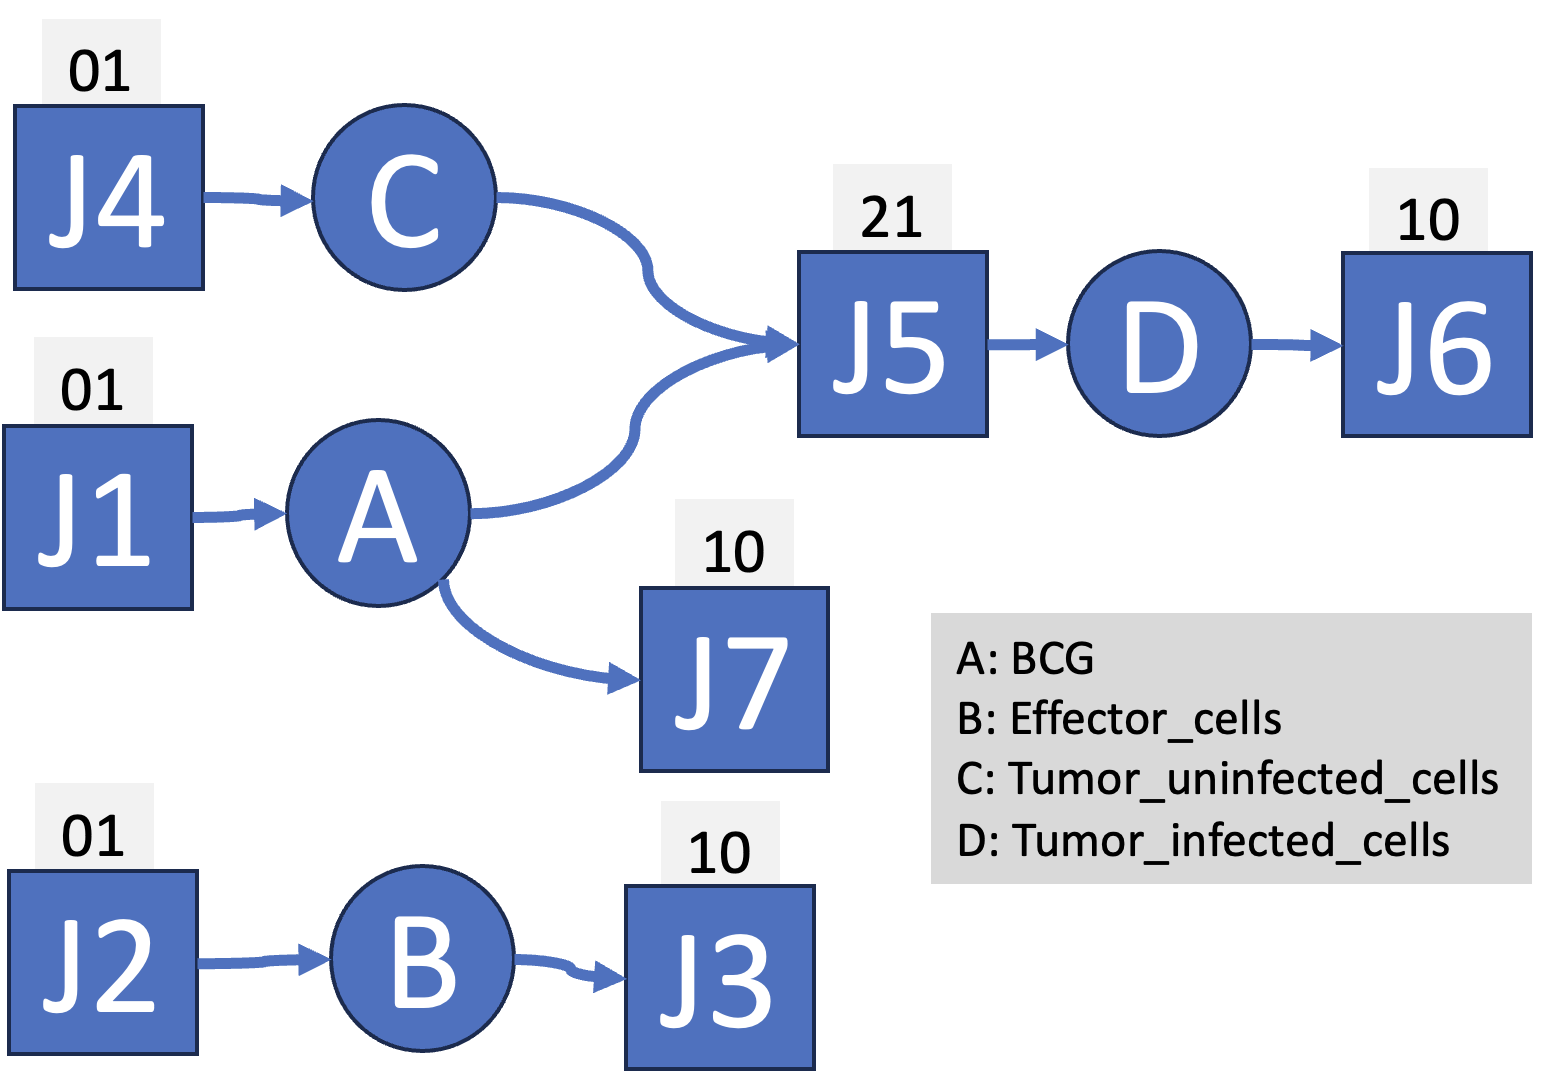
\includegraphics[width=1.25\textwidth, angle=0]{figures/bipartite-graph.png}
{\tiny {\bf (a) bipartite graph}}
\label{fig:bipartite-graph}
\end{minipage}
\hspace{0.5in}
%%
\begin{minipage}{0.9in}
%\begin{subfigure}{0.12\textwidth}
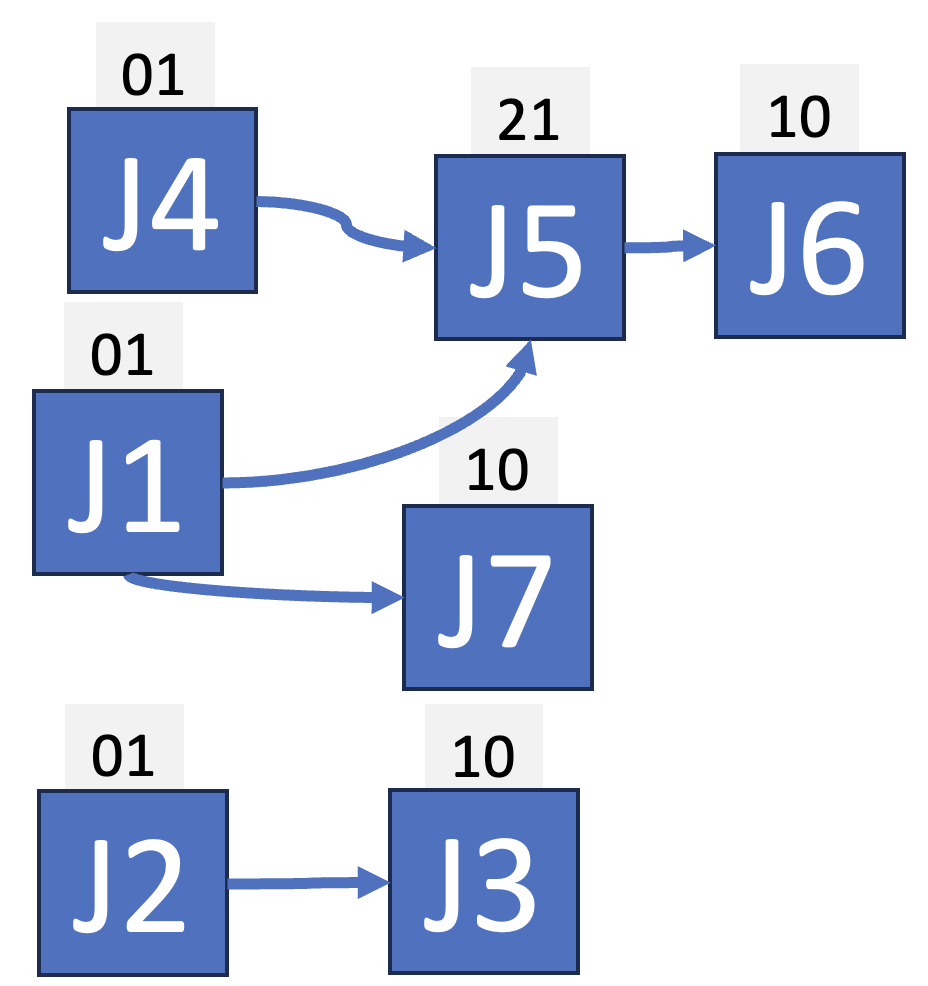
\includegraphics[width=1.25\textwidth, angle=0]{figures/monopartite-graph.png}
{\tiny {\bf (b) reaction monopartite graph}}
\label{fig:monopartite-graph}
\end{minipage}
%%
\caption{Bipartite graph and reaction monopartite graph for Model 1034.
Squares indicate reactions, and circles indicate species. Text above squares indicate the reaction type (e.g. 01 is 0 reactants, 1 product). The reaction monopartite graph is inferred from the bipartite graph.}
\label{fig:bipartite}
\end{figure}
%%%%%
 
 This problem can be avoided by representing CRNs as hypergraphs (e.g. \citep{yang_hgmatch_2023}). By so doing, reactions have two hyperarcs: (a) an inbound arc with a source at each reactant and a single destination at the reaction, and (b) an outbound arc whose single source is the reaction and whose destinations are each product species.
 For example, the bipartite graph in \fig{fig:bipartite}(a)
 has an inbound hyperarc for reaction \texttt{J5}
 with a source at its two reactants.
 The hypergraph representation avoids the problem described above because a target reaction is compatible with a reference reaction only if both reactions have the same number of reactants and products. 
 Almost all subgraph algorithms on hypergraphs find {\em similar} subgraphs, not subgraph isomorphisms. Similarity algorithms score reaction pairs in many ways such as counting types of subgraphs (e.g. feedforward loops) and commonalities in their participants (e.g. 6 carbon sugars)
\citep{zhang_h2mn_2021, sharan_modeling_2006, milano_challenges_2022}.
As a result, similarity algorithms often require species annotations, and they do not analyze the full topology of connections between species and reactions.


To our knowledge, only \citep{yang_hgmatch_2023} proposes an algorithm for finding subgraph isomorphisms in hypergraphs.
 Even better, this work discusses process-based parallelism (i.e. running on multiple processors) to speed up the computationally intensive processing of the subgraph problem.
 The authors employ a {\bf constraint-based approach}, such as only considering the mapping of a reference node to a target with at least as many incoming and outgoing arcs as the reference.
 However, \citep{yang_hgmatch_2023} is a general purpose algorithm, not an algorithm specifically targeted at CRNs. For example, the constraint they impose on the number of arcs is useless for reactions in CRNs since all reactions have a single incoming arc and a single outgoing arc.
 Further, they use  the same criteria for all nodes, but we need to use different criteria for reaction and species nodes.
 Beyond this, \citep{yang_hgmatch_2023} does not attempt computational speedup using vectorization (i.e., speedups achieved by using matrix representations instead of graph representations).
 Vectorization speedups can be substantial.
 For example, \secref{sec:parallelism} shows a speed increase of a factor of 40 by using vectorization.

This article introduces \py{}, an open source Python package that discovers subnets in CRNs represented using the community standard of systems biology markup language (SBML) \citep{hucka_systems_2003}.
\py{} employs a constraint-based approach that greatly reduces computations.
\revision{In our studies of randomly selected target networks with
100 reaction that each embed a random reference networks with 20 reactions, the number of mapping pairs is reduced from
a computationally infeasible $10^{78}$ to a more practical $10^{8}$.}
Furthermore, our implementation provides large speedups as a result of vectorization and process-based parallelism
(e.g. a speedup of 400 in our studies).
In addition, we develop a methodology that assesses the statistical significance of subnet discovery.
Last, we use \py{} to study subnets in BioModels
for approximately 200,000 pairs of reference and target models.
We show that for a reference MAPK pathway, subnet discovery correctly indicates the presence of MAPK function in several target models.
The studies also suggest a couple of interesting hypotheses: (a) the potential presence of hidden oscillators in several models in BioModels,
and (b) the possibility of a conserved mechanism for intracellular immune response.


%%%%%%%%%%%%%%%%%%%%%
\section{Methods}
\py{} draws on previous work on constraints-based approaches
to subgraph problems, and leverages
an analysis of the distribution of reactions in BioModels.

%%%%%
\begin{figure}[hbtp]
\centering
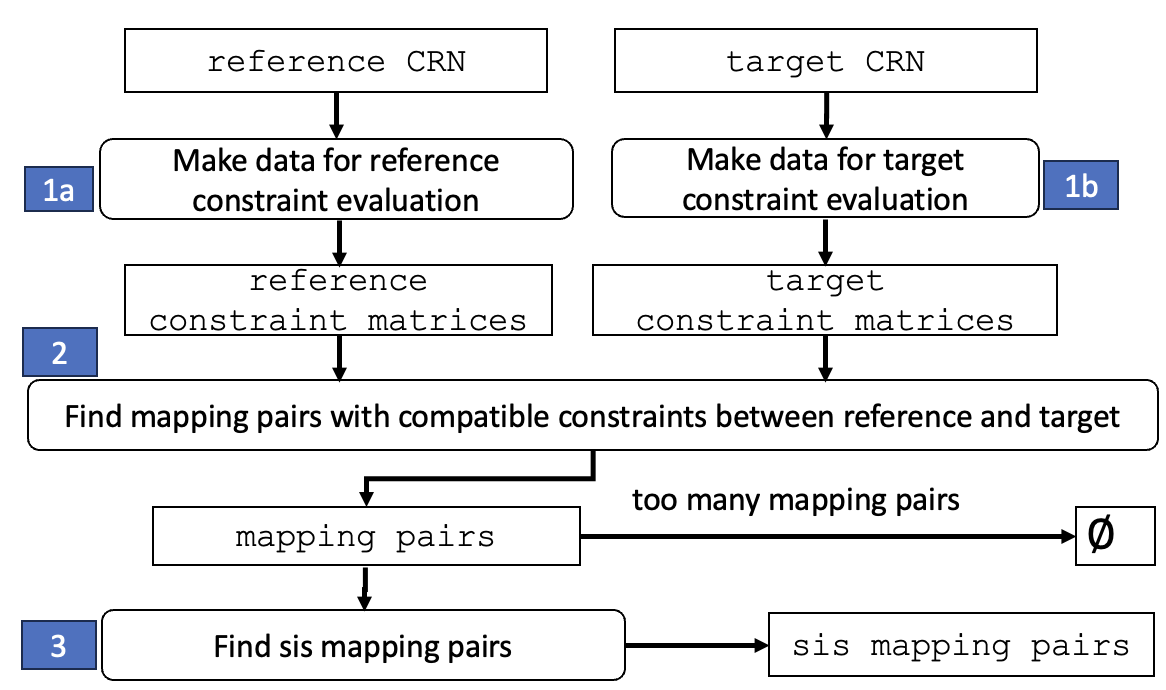
\includegraphics[width=0.35\textwidth, angle=0]{figures/program-logic.png}
%{\tiny
%    \begin{adjustbox}{padding=15pt 0pt 0pt 0pt, fbox}
%    \begin{lstlisting}[language=Mathematica, numbers=left, numbersep=4pt]
%def findSubnets(reference:Network, target:Network, identity:Enum, max_num_mappings:int)
%    # Construct mapping pairs
%    mapping_pairs = %makemappingPairs(reference.constraints, %target.constraints)
%    if len(mapping_pairs) > max_num_mappings:
%        return empty_set
%    # Find mappings that identify an induced network in %the target
%    mapping_pairs = []
%    parallelfor mapping_pair in mapping_pairs
%        if identity == weak
%            if reference.standard_mat = target.standard_mat(asignment_pair)
%               mapping_pairs.append(mapping_pair)
%        else /* identity == strong */
%            if reference.reactant_mat = target.reactant_mat(asignment_pair) and
%                 reference.product_mat = target.product_mat(asignment_pair)
%                mapping_pairs.append(mapping_pair)
%    return mapping_pairs
%               
%    \end{lstlisting}
%    \end{adjustbox}
    \caption{High level algorithm for subnet discovery. Data are indicated by regular rectangles. Program logic is indicated by rounded rectangles and annotated with shaded numbers to indicate the sequence of steps.}
    \label{fig:program-logic}
%}
\end{figure}
%%%%%

\subsection{Constraint-Based Subnet Discovery}
\fig{fig:program-logic} displays our high-level algorithm for subnet discovery.
Processing steps are indicated by rectangles with rounded edges, and data by rectangles with unrounded edges and text in a teletype font. Steps 1a and 1b construct constraints for the reference and target CRNs.
Step 2 uses constraints to find a subset of mapping pairs that are potentially inferred networks in the target that are structurally identical to the reference.
Step 3 evaluates mapping pairs to find sis mapping pairs.

The high-level program logic in \fig{fig:program-logic} is quite similar to \citep{yang_hgmatch_2023}.
However, we proceed in a different way.
First, we use constraints that are specific to the characteristics of CRNs,
especially the nature of incoming and outgoing hyperarcs for reactions in CRNs.
Second, we use matrix representations of constraints and the chemical network to achieve speedups through vectorization.
Third, we provide a way to manage the "computational budget" by having a threshold on the number of mapping pairs that are evaluated.
These points are addressed in detail in
\secref{sec:results}.

%%%%%%%%%%%
\subsection{Generating Random CRNs}\label{sec:random-crn}
Our choice of constraints and the way in which we evaluate our algorithms are based on a statistical characterization of CRNs in the
BioModels repository \citep{xu_sbmlkinetics_2023}.
The characterization focuses on reactions and the observation that
a reaction can be classified by two numbers: its number of reactants
(the sources for the reaction's incoming arc)
and its number of products (destinations for its outgoing arc).
These two numbers constitute the {\bf reaction type}.
For example, a $(1, 2)$ reaction has 1 reactant species and two product species, such as $A \rightarrow B + C$.
\citep{xu_sbmlkinetics_2023} defines 16
reaction types, and
describes the distribution of
reaction types in BioModels.
In \py{}, the method
\texttt{NetworkBase}\texttt{.makeRandomNetworkByReactionType}
in the module \texttt{network\_base}
implements the random generation of CRNs according to this distribution.

The evaluation of subnet discovery requires generating reference-target pairs, where the reference is randomly embedded in the target. Our approach is implemented in the 
\texttt{network\_base} method \texttt{NetworkBase.RandomReferenceAndTarget}.
This
method inputs the size of the reference CRN,
$M^R_s$ species and $M^R_r$ reactions, 
and the size of the target CRN,
$M^T_s$ species and $M^T_r$ reactions.
The first step
constructs a
preliminary target CRN with $M^T_r - M^R_r$ reactions and
$M^T_s$ species.
Next,
the reference CRN is generated with
$M^R_r$ reactions and $M^R_s$ species using
species that are
randomly selected from the preliminary target CRN.
Lastly, the target network is constructed by merging (and randomizing) the preliminary target network with a copy of the reference network.


%%%%%%%%%%%%%%%%%%%%%%%%%%%%%%%%%%%%%%%%%%%%%%%%%%
\section{Results}\label{sec:results}
Here we discuss the CRN-specific constraints that
we employ (\secref{sec:constraints}), their effectiveness in reducing computational complexity (\ref{sec:effectivness-of-constraints}), how we use vectorization and process-based
parallelism and the speedups achieved (\secref{sec:parallelism}), and our approach to evaluating the statistical
significance of subnet discovery (\secref{sec:significance}).
\secref{sec:package} provides details of the package \py{}.


%%%%%%%%%%%%%%%%%
\subsection{Constraints for CRNs}\label{sec:constraints}

%%%%%%%%FIGURE%%%%%%%%%%%%%%%%
\begin{figure*}
%\begin{minipage}{0.95in}
%\begin{subfigure}{0.13\textwidth}
%{\tiny
%\begin{tabular}{|c|c|c|c|c|}
%\hline
%ID & type & \#10 & \#21 & \#11 \\
%\hline\hline
%J1 & 01 & 1 & 1 & 0 \\
%J2 & 01 & 1 & 0 & 0 \\
%J3 & 10 & 0 & 0 & 0 \\
%J4 & 01 & 0 & 1 & 0 \\
%J5 & 21 & 1 & 0 & 0 \\
%J6 & 10 & 0 & 0 & 0 \\
%J7 & 10 & 0 & 0 & 0 \\
%\hline
%\end{tabular}
%}
%{\tiny {\bf (a) constraints: 1034}}
%\end{minipage}
%\hfill
%%%
%\begin{minipage}{0.9in}
%%\begin{subfigure}{0.13\textwidth}
%{\tiny
%\begin{tabular}{|c|c|c|c|c|}
%\hline
%ID & type & \#10 & \#21 & \#11 \\
%\hline\hline
%v01 & 21 & 1 & 0 & 1 \\
%v02 & 21 & 1 & 0 & 1 \\
%v03 & 10 & 0 & 0 & 0 \\
%v04 & 10 & 0 & 0 & 0 \\
%v05 & 10 & 0 & 0 & 0 \\
%v06 & 10 & 0 & 0 & 0 \\
%v07 & 11 & 1 & 1 & 0 \\
%v08 & 11 & 1 & 1 & 0 \\
%v09 & 10 & 0 & 0 & 0 \\
%v10 & 01 & 1 & 1 & 0 \\
%v11 & 01 & 1 & 1 & 0 \\
%v12 & 01 & 1 & 0 & 0 \\
%\hline
%\end{tabular}
%}
%{\bf {\tiny (b) constraints: 351}}
%\end{minipage}
%\hfill
%%%
%\begin{minipage}{1.3in}
%\vspace{20pt}
%{\tiny
%\begin{tabular}{|c|l|}
%\hline
%1034 ID & compatible 351 IDs \\
%\hline\hline
%J1 & v10, v11\\
%J2 & v10, v11, v12 \\
%J3 & v03, v04, v05, v06, v07, v08, v09 \\
%J4 & v10, v11\\
%J5 &  v01, v02 \\
%J6 & v03, v04, v05, v06, v07, v08, v09 \\
%J7 & v03, v04, v05, v06, v07, v08, v09 \\
%\hline
%\end{tabular}
%}
%\newline
%{\tiny {\bf (c) compatibility collection}}
%\end{minipage}
%\hfill
%%%
%\begin{minipage}{1.4in}
%\vspace{20pt}
%{\tiny
%\begin{tabular}{|c|c|c|c|}
%\hline
%1034 ID & 1 & 2 & 3 \\
%\hline\hline
%J1 & v10 & v10 & v10 \\
%J2 & v12 & v12 & v12 \\
%J3 & v03 & v03 & v09 \\
%J4 & v11 & v11 & v11 \\
%J5 & v01 & v01 & v01 \\
%J6 & v04 & v06 & v05 \\
%\hline
%\end{tabular}
%}
%\vspace{0.2in}
%{\tiny {\bf (d) three reaction mappings}}
%\end{minipage}
%\hfill
%%
\centering
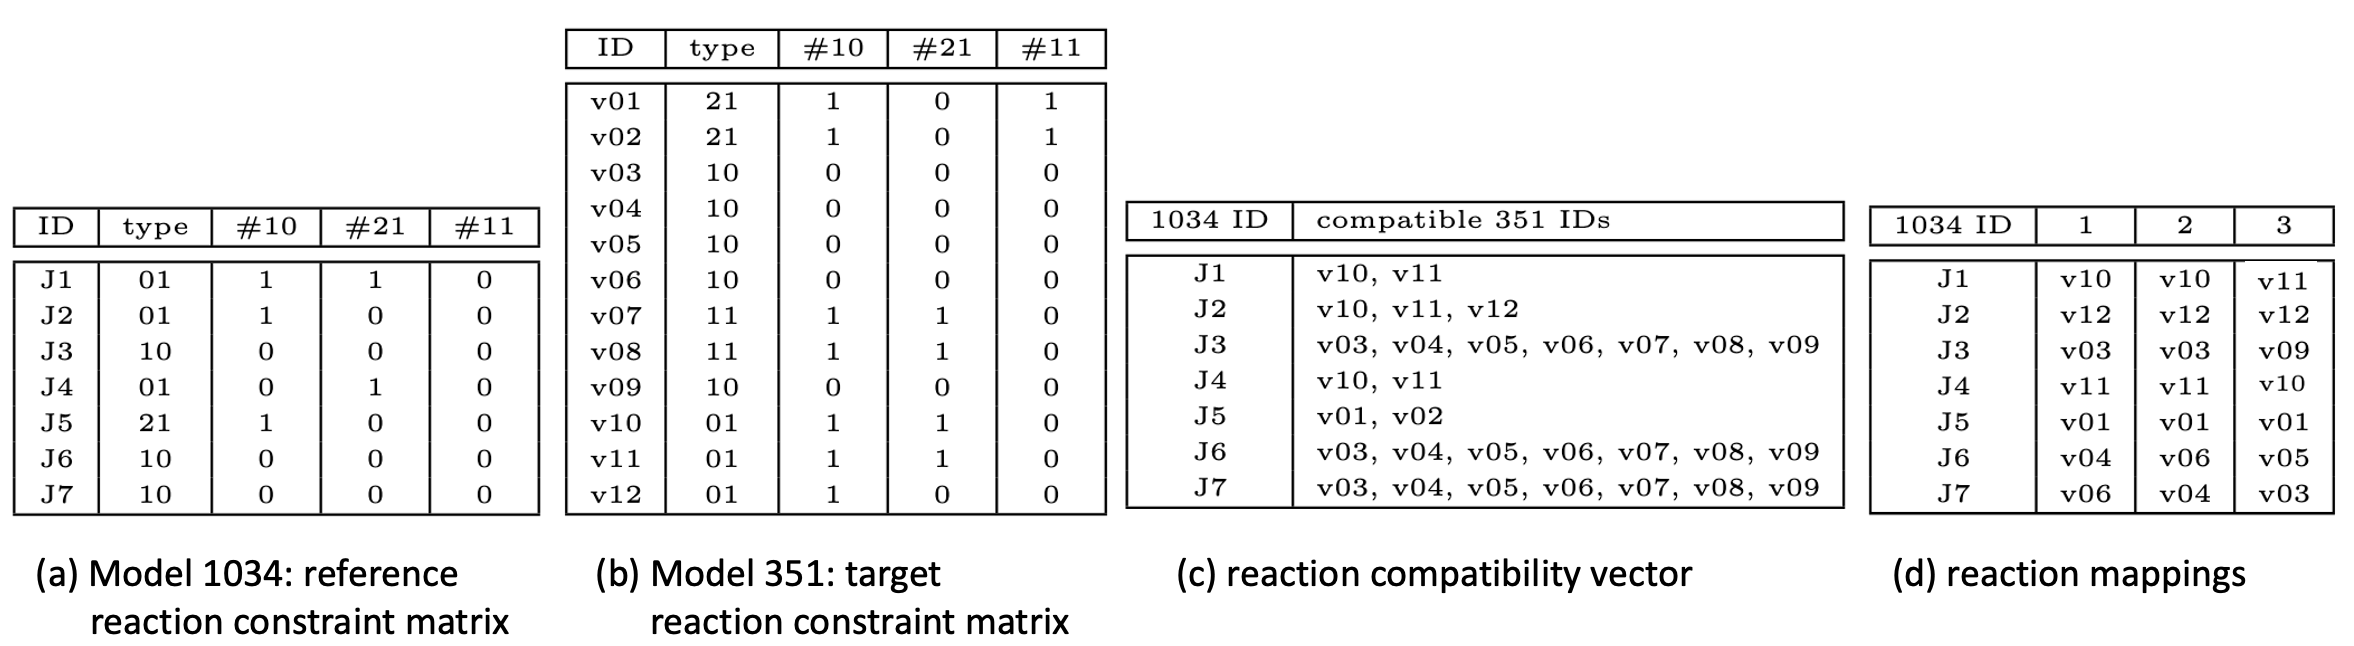
\includegraphics[width=0.85\textwidth,angle=0]{figures/constraint-data.png}
\caption{\revision{Illustration of calculating} reaction mappings.
(a) and (b) are partial data for reaction constraint matrices (reaction type, 1-step successor counts).
(c) is the reaction compatibility \revisionb{calculated from (a) and (b)}. (d) displays three reaction mappings (the columns) \revision{of the many reaction mappings; the reaction mappings are based on (c) and are obtained by selecting a unique 351 reaction in the list of compatible reactions for each 1034 reaction.}}
\label{fig:calculating-reaction-mappings}
\end{figure*}
%%%%%%%%FIGURE%%%%%%%%%%%%%%%%

\py{} employs a constraint-based approach to reduce the number of mapping pairs.
Constraints are custom-made to CRNs in two ways.
First, different constraints are used in the construction of reaction mappings and species mappings
(an approach that does not seem to be applied in other subgraph discovery algorithms).
Second, many of our constraints are structured using the concept of reaction type discussed in \secref{sec:random-crn}, something specific to CRNs.

%The \py{} constraint system is designed with extensibility in mind. Details are in the classes \texttt{ReactionConstraint} and \texttt{SpeciesConstraint}.

%%%%%%
\subsubsection{Reaction Constraints and Reaction Mappings}
Let $r^R$ be a reaction in the reference CRN and
$r^T$ be a reaction in the target CRN.
A constraint is a predicate (that is, a boolean-valued function) on $(r^R, r^T)$ such that: (a)
the result is always true if there is a sis mapping pair
with $r^R$ mapped to $r^T$
and (b) the result is false as frequently as possible
if there is no such sis mapping pair.
Put differently, constraints should have no false negative, and
constraints should minimize false positives (since false positive increase computation time).
%Constraints address the question ``Should $r^T$ be associated with $r^R$ in a reaction mapping?" We want to find predicates on $r^R, r^T$ such that: (a) we answer {\em always} "Yes" when $r^T$ should be associated with $r^R$ and (b) we answer "No" as frequently as possible if $r^T$ should {\em not} be associated with $r^R$ (so that we reduce the number of reaction mappings).

Our first reaction constraint, RC1, is that $r^T$ and $r^R$ must be the same reaction type.
For example, this constraint holds for $r^{R} = \texttt{J5}$ in Model \revision{1034}  in \fig{fig:running-example-models}(\revisionb{b}) and
$R^T = \texttt{v01}$ because both reactions have
two reactants and one product.
Note that to simplify the tables, we encode the reaction type using
two decimal digits so that $(2, 1)$ is represented as ``21".
%(\py{} uses a 4 digit representation, two digits for reactants, and two for products.)

The remaining constraints make use of the reaction monopartite graph, a graph in which all nodes are reactions.
This graph is constructed
from the full CRN bipartite hypergraph
by placing an arc from a source reaction to a destination reaction if the source has a product species that is a reactant for the destination.
\fig{fig:bipartite} displays the reaction monopartite graph for Model 1034.

Reaction constraints RC2 and RC3 use information about predecessors and successors in the reaction monopartite graph.
Consider \revision{the arc from reaction $J_1$ to $J_5$ in
\fig{fig:bipartite}(b).
Here, $J_1$ is a 1-step predecessor to $J_5$, and $J_5$} is a 1-step successor to $J_1$.
A 2-step predecessor is a predecessor of a 1-step predecessor,
and similarly for a 2-step successor.

The reaction constraints are the following.
\begin{itemize}
    \item RC1: $r^R$ and $r^T$ have the same reaction type.
    \item RC2: The count of 1-step and 2-step {\em predecessor} reactions (by type) for $r^R$ is no larger than the same count for $r^T$.
    \item RC3: The count of 1-step and 2-step {\em successor} reactions (by type) for $r^R$ is no larger than the same count for $r^T$.
\end{itemize}

Each CRN has a reaction and a species {\bf constraint matrix} that are constructed in Steps 1a, 1b in \fig{fig:program-logic}.
These matrices are used to evaluate constraints when constructing mapping pairs (step 2 in \fig{fig:program-logic}).
A row in the reaction constraint matrix corresponds to a
reaction, and columns provide data used in constraint evaluations.
There is a column for RC1 (reaction type).
For RC2, there are two columns for each possible predecessor reaction type; cell values indicate the number of 1-step and 2-step predecessor reactions for the reaction type.
Similarly, there are two columns for each reaction type for RC3.
\fig{fig:calculating-reaction-mappings}(a) and
\fig{fig:calculating-reaction-mappings}(b)
display portions of
the reaction constraint matrices for 1034 and 351, respectively.
The columns RC2 and RC3 contain counts and are labeled with a hash (``\#") followed by a reaction type (encoded as a two-digit integer).

The construction of the reaction mappings involves building
the {\bf reaction compatibility vector}.
The vector's $i^{th}$ position is for the
$i^{th}$ reference reaction
and contains
the set of reactions in the
target that can be associated with the $i^{th}$ reference reaction
(based on evaluating RC1-RC3).
\fig{fig:calculating-reaction-mappings}(c) \revision{displays
the reaction compatibility vector using the constraints 
in \fig{fig:calculating-reaction-mappings}(a) and
\fig{fig:calculating-reaction-mappings}(b).
\fig{fig:calculating-reaction-mappings}(d) shows three of the many reaction mappings obtained from
\fig{fig:calculating-reaction-mappings}(c) by
selecting a distinct 351 reaction in the list of compatible reactions for each 1034 reaction.}
%For example, \texttt{J1} in 1034 is compatible with \texttt{v10} and \texttt{v11} because (i) the latter two have the same reaction type as \texttt{J1} (``01") and (ii) the other constraint columns for \texttt{J1} are no larger than the corresponding constraint columns for \texttt{v10} and \texttt{v11}.

A reaction mapping is constructed by selecting one target reaction
from each entry in the reaction compatibility vector without repeating a target reaction.
\fig{fig:calculating-reaction-mappings}(d) illustrates three reaction mappings for the running example.
%Note that an upper bound on the number of reaction mappings is the product of the length of each entry in the compatibility vector.

%%%%%
\begin{figure}
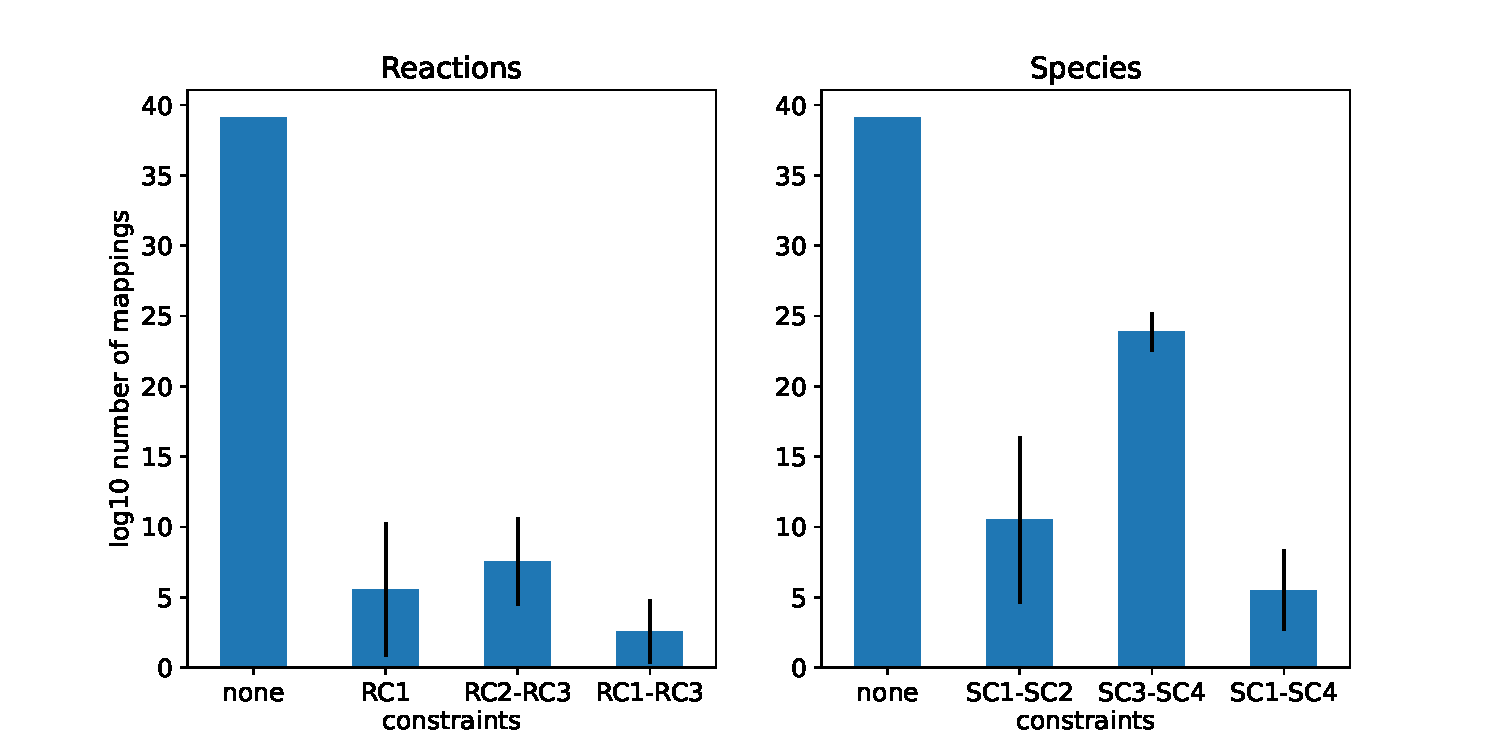
\includegraphics[width=0.5\textwidth, angle=0]{figures/evaluate_constraints.pdf}
\caption{Constraints reduce the number of mappings to be evaluated by over $10^{30}$ for both species and reactions. The plots report the $log_{10}$ of the number of mappings to be evaluated for combinations of constraints. Solid bars are median values from simulation studies, and vertical lines indicate sample standard deviations.}
\label{fig:constraint-effectiveness}
\end{figure}
%%%%%

%%%%%
\begin{figure}
\hspace{-.4in}
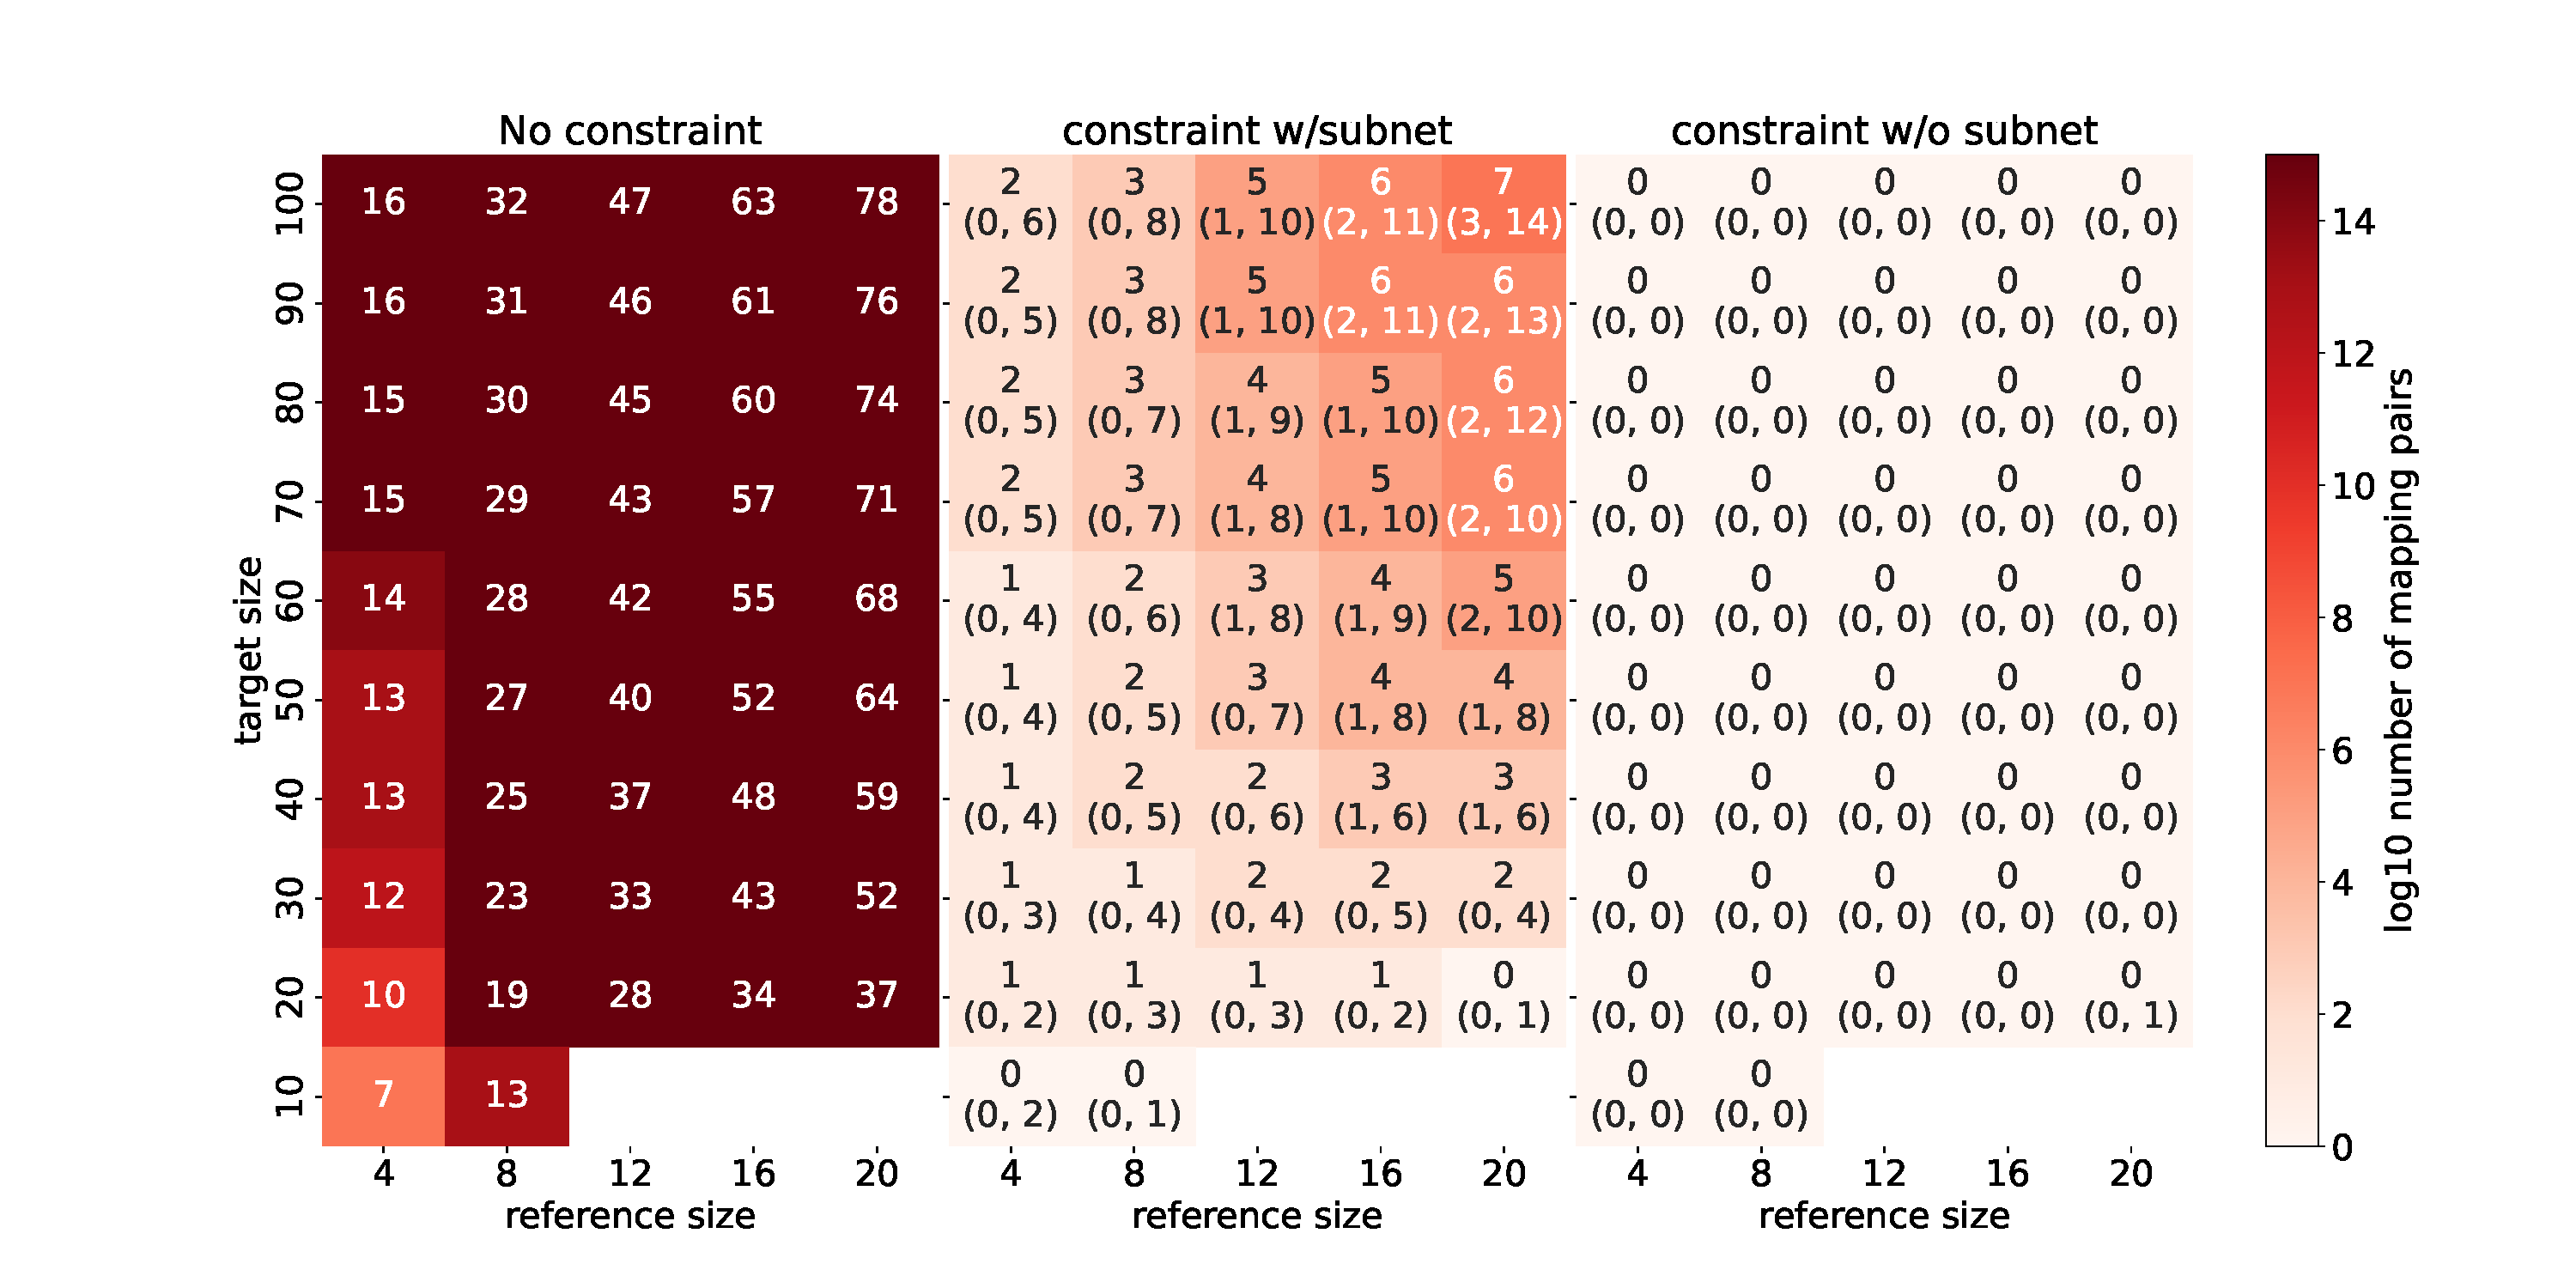
\includegraphics[width=0.59\textwidth, angle=0]{figures/scalable_subnet_discovery.pdf}
\caption{Constraints reduce the number of mapping pairs to be evaluated when a reference network is present and even more when it is absent.
Unparenthesized numbers are the integer part $log_{10}$ of the median number of mappings of 1,000 simulations; parenthesized numbers are the 10\% and 90\% percentiles of 1,000 simulations.}
\label{fig:scalable-subnet-discovery}
\end{figure}
%%%%%

%%%%%
\subsubsection{Species Constraints and Species Mappings}
Species constraints are organized and implemented in a manner analogous
to reaction constraints.
There are species constraint matrices, species compatibility vectors, and species mappings obtained from species compatibility vectors.
%In addition, a species monopartite graph is inferred in the same way as the reaction monopartite graph; 1-step and 2-step successors and predecessors are defined as before for reactions. Species constraints may be equality or inequality constraints. Initially, we had a single equality constraint for species to indicate if a species appears as both a reactant and product in the same reaction. Our evaluations of the effectiveness of the constraint indicate that this constraint did little to limit the number of species mappings; so it was eliminated.

Species are based on
the full CRN bipartite graph.
Let $s^R$ be the reference species and $s^T$ be the target species.
The species constraints check that $s^T$ is referenced in reactions at least as often as $s^R$ is referenced.
\begin{itemize}
    \item SC1: The count of reactions (by type) in which $s^R$ is a {\em reactant} does not exceed the corresponding count for $s^T$.
    \item SC2: The count of reactions (by type) in which the $s^R$ is a {\em product} does not exceed the corresponding count for $s^T$.
     \item SC3: The count of reactions (by type) that can be reached by $s^R$ within 2 steps in the {\em forward} direction does not exceed the same count for $s^T$.
     \item SC4: The count of reactions (by type) that can be reached by $s^R$ within 2 steps in the {\em reverse} direction does not exceed the same count for $s^T$.
\end{itemize}

%%%%%%%%%%%%%%%%%%%
\subsection{Effectiveness of Constraints}\label{sec:effectivness-of-constraints}
We quantify the effectiveness of reaction and species constraints by reducing reaction and species mappings.
Our studies calculated the number of mappings for different combinations of constraints.
For reactions, we considered the conditions: (i) no constraints (none),
(ii) only RC1, (iii) only RC2 and RC3, and (iv) all constraints (RC1-RC3).
For species, the conditions are: (i) no constraints, (ii) SC1-SC2,
(iii) SC3-SC4, and (iv) SC1-SC4.
Condition (i) (reactions and species) is calculated deterministically as in
\eqnref{eq:naive}.
The remaining conditions are evaluated using 1,000 iterations
of random networks.
An iteration for reaction (species) constraints considers one of conditions
(ii)-(iv).
We use \secref{sec:random-crn} to generate a random target CRN with 100 reactions and 100 species that has a subnet that is the reference with 20 reactions and 20 species.
Then, we execute steps 1a, 1b, and 2 in \fig{fig:program-logic} for reactions (species), and count the number of reaction (species) mappings using the method
\texttt{CompatibilityCollection.}
\linebreak
\texttt{log10\_num\_assignment}
in the \py{} module
\linebreak
\texttt{compatibility\_collection.py}.

\fig{fig:constraint-effectiveness} displays a bar plot of the results of these studies.
The vertical axis is the number of mappings in units $log_{10}$, and
the horizontal axis indicates combinations of constraints (conditions).
The vertical lines are standard deviations.
If no constraint is applied, the number of mappings is very close to $10^{40}$ for both reactions and species, and so
is almost $10^{80}$ mapping pairs (the product of the number of species and reaction mappings).
Applying all constraints in combination, we have approximately $10^3$ mappings for reactions and $10^5$ mappings for species, or $10^8$ mapping pairs.
This is a reduction by a factor of more than $10^{70}$ in the number of mapping pairs compared to the number that does not have constraints.

\fig{fig:scalable-subnet-discovery} uses the same procedure as above to study the number of mapping pairs under three conditions: (a) no constraints; (b) all constraints when the reference is present in the target; and (c) all constraints when the reference is not present in the target.
Cells are annotated with the integer part of $log_{10}$ of the number of mapping pairs obtained from the simulation; numbers in parentheses are the $10^{th}$ and $90^{th}$ percentiles obtained from simulation.
(Parenthesized numbers are not needed for ``no constraint" since this is
a deterministic calculation.)
The reference size is the horizontal axis; the target size is the vertical axis; darker colors indicate a larger number of mapping pairs.
We see that constraints provide a huge reduction in mapping pairs, even for larger references and targets.
Also of note is the effectiveness of constraints in detecting the {\em absence} of the reference in the target.
We see that for this condition and with very large CRNs, the number of mapping pairs is quite small.
    
%%%%%%%%%%%%%%%%%%%%%%%%%
\subsection{Computational speedups}\label{sec:parallelism}
Constraints dramatically reduce the number of mapping pairs. 
However, even after constraints are applied, there may still be $10^{10}$ to $10^{13}$ mapping pairs.
The evaluation of these many mapping pairs requires considerable computation.

%The evaluation of an mapping pair requires comparing one or more stoichiometry matrices in the reference CRN with a permuted submatrix of one or more target stoichiometry matrices. For strong identity, comparisons are done for both the reactant and product stoichiometries; for weak identity, only the standard stoichiometry matrices are compared. When comparing stoichiometry matrices, the rows of the target sub-matrix are determined by the species mapping, and the columns by the species mapping.
\py{} achieves computational speedups in two ways.
The first approach is {\bf vectorization}, the use of matrix operations instead of executing \texttt{for} loops.
\py{} uses vectorization in the construction of mapping pairs
that comply with constraints
(step 2 in \fig{fig:program-logic})
and in the evaluation of mapping pairs
(step 3 in \fig{fig:program-logic}).
In particular,
the latter requires testing for equality between the reference stoichiometry matrix and the permuted subset of the target stoichiometry matrix specified by the mapping pair.
The foregoing can be done for one mapping pair at a time.
\py{} implements a scheme for stacking stoichiometry matrices so that $m$ mappings can be evaluated simultaneously.

We conducted studies measuring the runtime for stacking $m$ matrix comparisons in the evaluation of mapping pairs;
$m \in \{ 1, 10, 100, 1000 \}$.
The studies used randomly generated reference networks (5 reactions, 5 species) that were embedded in randomly generated target networks (100 reactions, 100 species) as described in \secref{sec:random-crn}.
Subnet discovery was done on one core of a 128 GB Mac Studio M1 with 20 cores.
Let $T_M(m)$ be the execution time for stacking $m$ stoichiometry matrices.
The speedup is $S_M(m) =\frac{T_M(1)}{T_M(m)}$.
The results indicated a substantial speedup from the use of vectorization:
$S_M(10) \approx 9, S_M(100) \approx 30, S_M(1000) \approx 40$. No significant improvement was observed for $m > 1000$.

\py{} also implements process parallelism using the Python \texttt{multiprocessing} package to take advantage of systems with multiple processors (cores).
As a result,
step 3 in \fig{fig:program-logic}
evaluates the mapping pairs in parallel on many processors.

%%%%%
\begin{figure}
\hspace{0.2in}
\centering
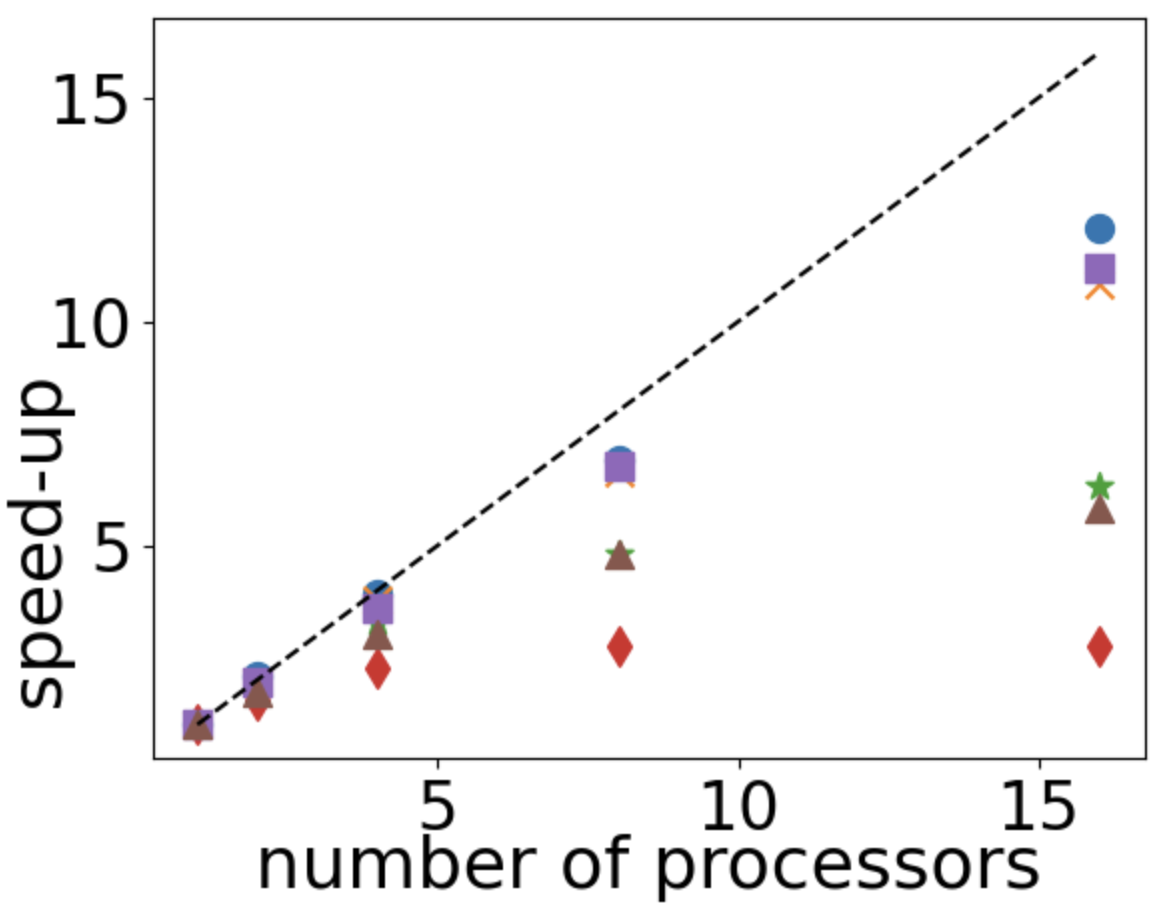
\includegraphics[width=0.2\textwidth, angle=0]{figures/speedup.png}
\caption{Speedup from process parallelism. Markers indicate studies. Speedups are larger when there are more mapping pairs.}
\label{fig:speedup}
\end{figure}
%%%%%

To assess the speedup for process parallelism, we conducted 6 studies with a different set of 10 random target CRNs (100 reactions, 100 species); each target CRN had an embedded reference CRN (5 reactions, 5 species). These networks were generated using the method in \secref{sec:random-crn}.
Then, subnet discovery was done using 1, 2, 4, 8, and 16 processors on a 128 GB Mac Studio M1 (with 20 cores).
Let $T_P(n)$ be the time for subnet discovery on $n$ processors.
The study calculated the speedup as $S_P(n) = \frac{T_P(1)}{T_P(n)}$.
\fig{fig:speedup} reports the results.
Marker shapes indicate speedups for different studies.
The dashed line is the ideal speedup, which is $S_P(n) = n$  or linear speedup.
We see that a near linear speed up is achieved in 3 of the studies (although less than linear for 16 processors).
As expected, a
near linear speed is achieved for studies with a large number of mapping pairs since there is more parallel work.

Computational speedups are multiplicative.
So, a speedup of 40 from vectorization and a speedup of 10 from process parallelism results in an overall speedup of 400.
That is, a subnet discovery that would take 1 day on a single processor evaluating one mapping pair at a time will instead have an elapsed of 3.5 minutes on 15 processors that use vectorization of 1,000 mapping pairs.

%%%%%%%%%%%%%%%%%%
\subsection{Statistical Significance of Subnet Discovery}\label{sec:significance}

%%%%%
\begin{figure}
\centering
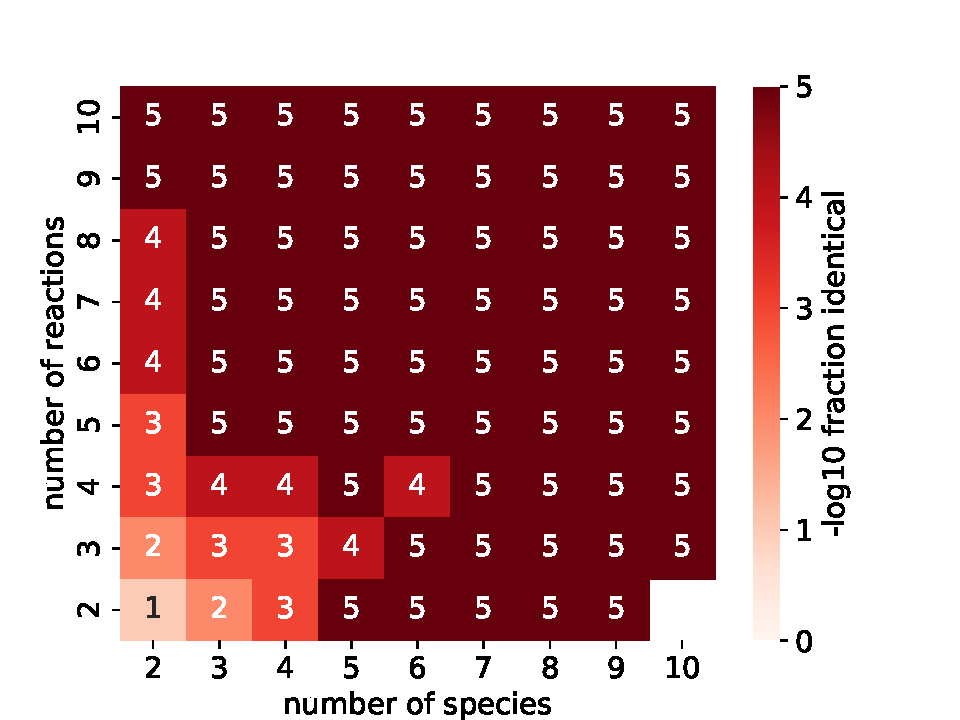
\includegraphics[width=0.3\textwidth, angle=0]{figures/poc_random_benchmark.pdf}
\caption{Statistical significance of randomly chosen CRNs.
Cells are annotated with $-log p$, where $p$ is the probability of a randomly chosen CRN as described in \secref{sec:significance}. The horizontal axis is the number of species, and the vertical axis is the number of reactions.
}
\label{fig:statistical-significance}
\end{figure}
%%%%%
Some CRNs are quite small. Since there are many more instances of small CRNs than larger ones, it is possible that the subnet discovery for a small CRN is not statistically significant.
%For example, BioModels 76 has 2 reactions and 3 species. A more extreme example is a CRN consisting of a single reaction. The foregoing motivates our desire to quantify the statistical significance of the discovery of subnets.

%The synthetic networks in \secref{sec:random-crn} can be used to quantify the statistical significance of subnet discovery Consider a reference CRN with $M^R_s$ species and $M^R_r$ reactions. We refer to {\bf network size} as the tuple $(M^R_s, M^R_t)$. Let the target CRN have size $(M^T_s, M^T_t)$. Suppose that there is an induced CRN in the target. An approach to evaluating statistical significance is to calculate how often a randomly chosen target of size $(M^T_s, M^T_r)$ contains the reference network. This is accomplished by repeatedly (a) choosing a random CRN of size $(M^T_s, M^T_t)$ and (b) performing subnet discovery with the reference CRN on this target. Since we are interested in the tail of the distribution and to allow for variability due to the random generation of targets, we need to repeat (a) and (b) a large number of times. In our studies, we used 100,000 repetitions. Thus, if an inferred CRN is found only once in 100,000 iterations, the discovery of a subnet is significant at the $10^{-5}$ level.

%The high computational cost of the above motivates a second approach.
We assess statistical significance by answering the question ``How likely is the reference CRN to occur by chance?"
This depends on the number of reactions and species in the reference, which are denoted by $(M^R_s, M^R_r)$.
We calculate the probability of ``occurring by chance" (null distribution)
using
randomly generated CRNs as described in \secref{sec:random-crn}.
\revision{
\begin{itemize}
    \item Step (1): generate $K^R$ reference CRNs with size $(M_s^R, M_r^R)$;
    \item Step (2): generate $K^T$ target CRNs also of size $(M_s^R, M_r^R)$;
    \item Step (3): for each reference CRN in step (1), count the number of target CRNs in step (2) that are strongly structurally identical, and report the fraction of occurrences of strong structural identity.
\end{itemize}
$K^R$, $K^R$ should be sufficiently large so that there is little variability for the statistics
calculated in step (3).
We find that it is sufficient to use $K^R = 100, K^T=1000$.}
%for different combinations of the number of reactions and number of species This second approach focuses on the reference CRN in isolation by evaluating how frequently a randomly chosen network with size $(M^R_s, M^R_r)$ is structurally identical to the reference CRN. This approach would seem to {\em underestimate} the significance of an inferred CRN, since the first approach considers more possible networks (as suggested by \eqnref{eq:naive}). However, we find that the two approaches generally provide comparable significance levels. In addition, the second approach turns out to provide a simple rule of thumb for statistical significance, which is presented below.

\fig{fig:statistical-significance} displays the result of the above approach for network sizes from $(2, 2)$ to $(10, 10)$.
The horizontal axis is the number of species in the model, and the vertical axis is the number of reactions.
Cells are annotated with the integer part of $-log_{10}$ of the fraction of random CRNs that are strongly identical under the null distribution (i.e., the Type 1 error in statistical inference \citep{lindgren_1993}).
For example, an annotation of "1" means a significance level of 0.1.
(A "5" means that the step found either 1 or 0 structurally identical networks.)
In the sequel, we use \fig{fig:statistical-significance} to evaluate the statistical significance.
%Note that statistical significance is not symmetric with respect to the number of species and reaction.
%Specifically, a network with two species is more likely to occur by chance than a network with two reactions.

%We use \fig{fig:statistical-significance} in two ways. The first is to construct a rule of thumb: The discovery of subnets is statistically significant if the induced network has at least 4 species and 4 reactions (since all such subnets in the figure are significant at the $10^{-5}$ level). A second technique uses \fig{fig:statistical-significance} directly. For example, BioModels 76 with 2 reactions and 3 species is significant at the 0.01 level.

%In theory, constructing \fig{fig:statistical-significance} requires massive computation, several million invocations of an algorithm for finding structurally identical networks (e.g. \py{}, \texttt{nauty}). However,  significant speedups are achieved by using a special purpose hash of stoichiometry matrices to detect structural identity (since structural identity is equivalent to there being a permutation of rows and columns that make the two matrices identical). Details of this hash are in the \py{} utility function \texttt{util.hashMatrix}.
%We note that our approach to statistical significance underestimates the probability of the occurrence of a reference CRN in the target. A more accurate alternative is to use the actual target CRN in Step (2). However, doing so requires a calculation for each assessment of statistical significance. Fortunately, it turns out that this alternative gives very close to the same results as in \fig{fig:statistical-significance}.

%%%%%%%%%%%
\subsection{Python Package}\label{sec:package}

\py{} is an open source Python package.
Models can be represented in the SBML (XML) or in the human-readable Antimony model description language \citep{smith_antimony_2009}.
The package is installed using
\texttt{pip install pySubnetSB}.

The basic API consists of two functions.
The first is
\texttt{findReferenceInTarget} that takes three arguments:
\linebreak
\texttt{reference\_model}, \texttt{target\_model}, and
    \texttt{max\_num\_mapping\_pair}.
The reference model is the
first argument, and the target model is the second argument.
The function returns an indicator of whether subnet discovery was aborted
because the number of mapping pairs exceeded  \texttt{max\_num\_mapping\_pair}.
The second API is \texttt{findReferencesInTargets}, which generalizes the first API to do subnet discovery for directories of models. 
%reference-target pairs for reference models in \texttt{reference\_directory} (first argument) and target models in \texttt{target\_directory} (second argument). This function also includes the argument \texttt{max\_num\_mapping\_pair}.
More details
can be found in the Jupyter notebook
\texttt{api\_basics.ipynb} in \url{https://github.com/ModelEngineering/pySubnetSB/blob/main/examples/}.
%The notebook can be executed by uploading it to Google Drive and using Google Colab.

%%%%%%%%%%%%%%%%%%%%%%%%%%%
\section{Application to BioModels}\label{sec:biomodels}

%%%%%
\begin{figure}
{\tiny
\begin{tabular}{|l|r|r|}
\hline
statistic & weak & strong \\
& identity & identity \\
\hline\hline
number of reference models processed & 223 & 224 \\
number of target models processed & 489 & 489 \\
number of pairs evaluated & 94,030 & 109,536 \\
number of \revision{inferred} subnets & 1338 & 1212 \\
number of reference models in \revision{inferred} subnets & 93 & 83 \\
number of target models with \revision{inferred} subnets & 328 & 274 \\
processing time & 6.7 hr & 6.9 hr \\
%time to process & 8.5 hr & 8.25 hr \\
\hline
\end{tabular}
}
\caption{Summary of subnet discovery for curated BioModels.}
%Reference models had no more than 10 reactions; target models had at least 10 reactions.}
\label{fig:biomodels-summary}
\end{figure}
%%%%%

%%%%%
%\begin{figure}
%\hspace{-.2in}
%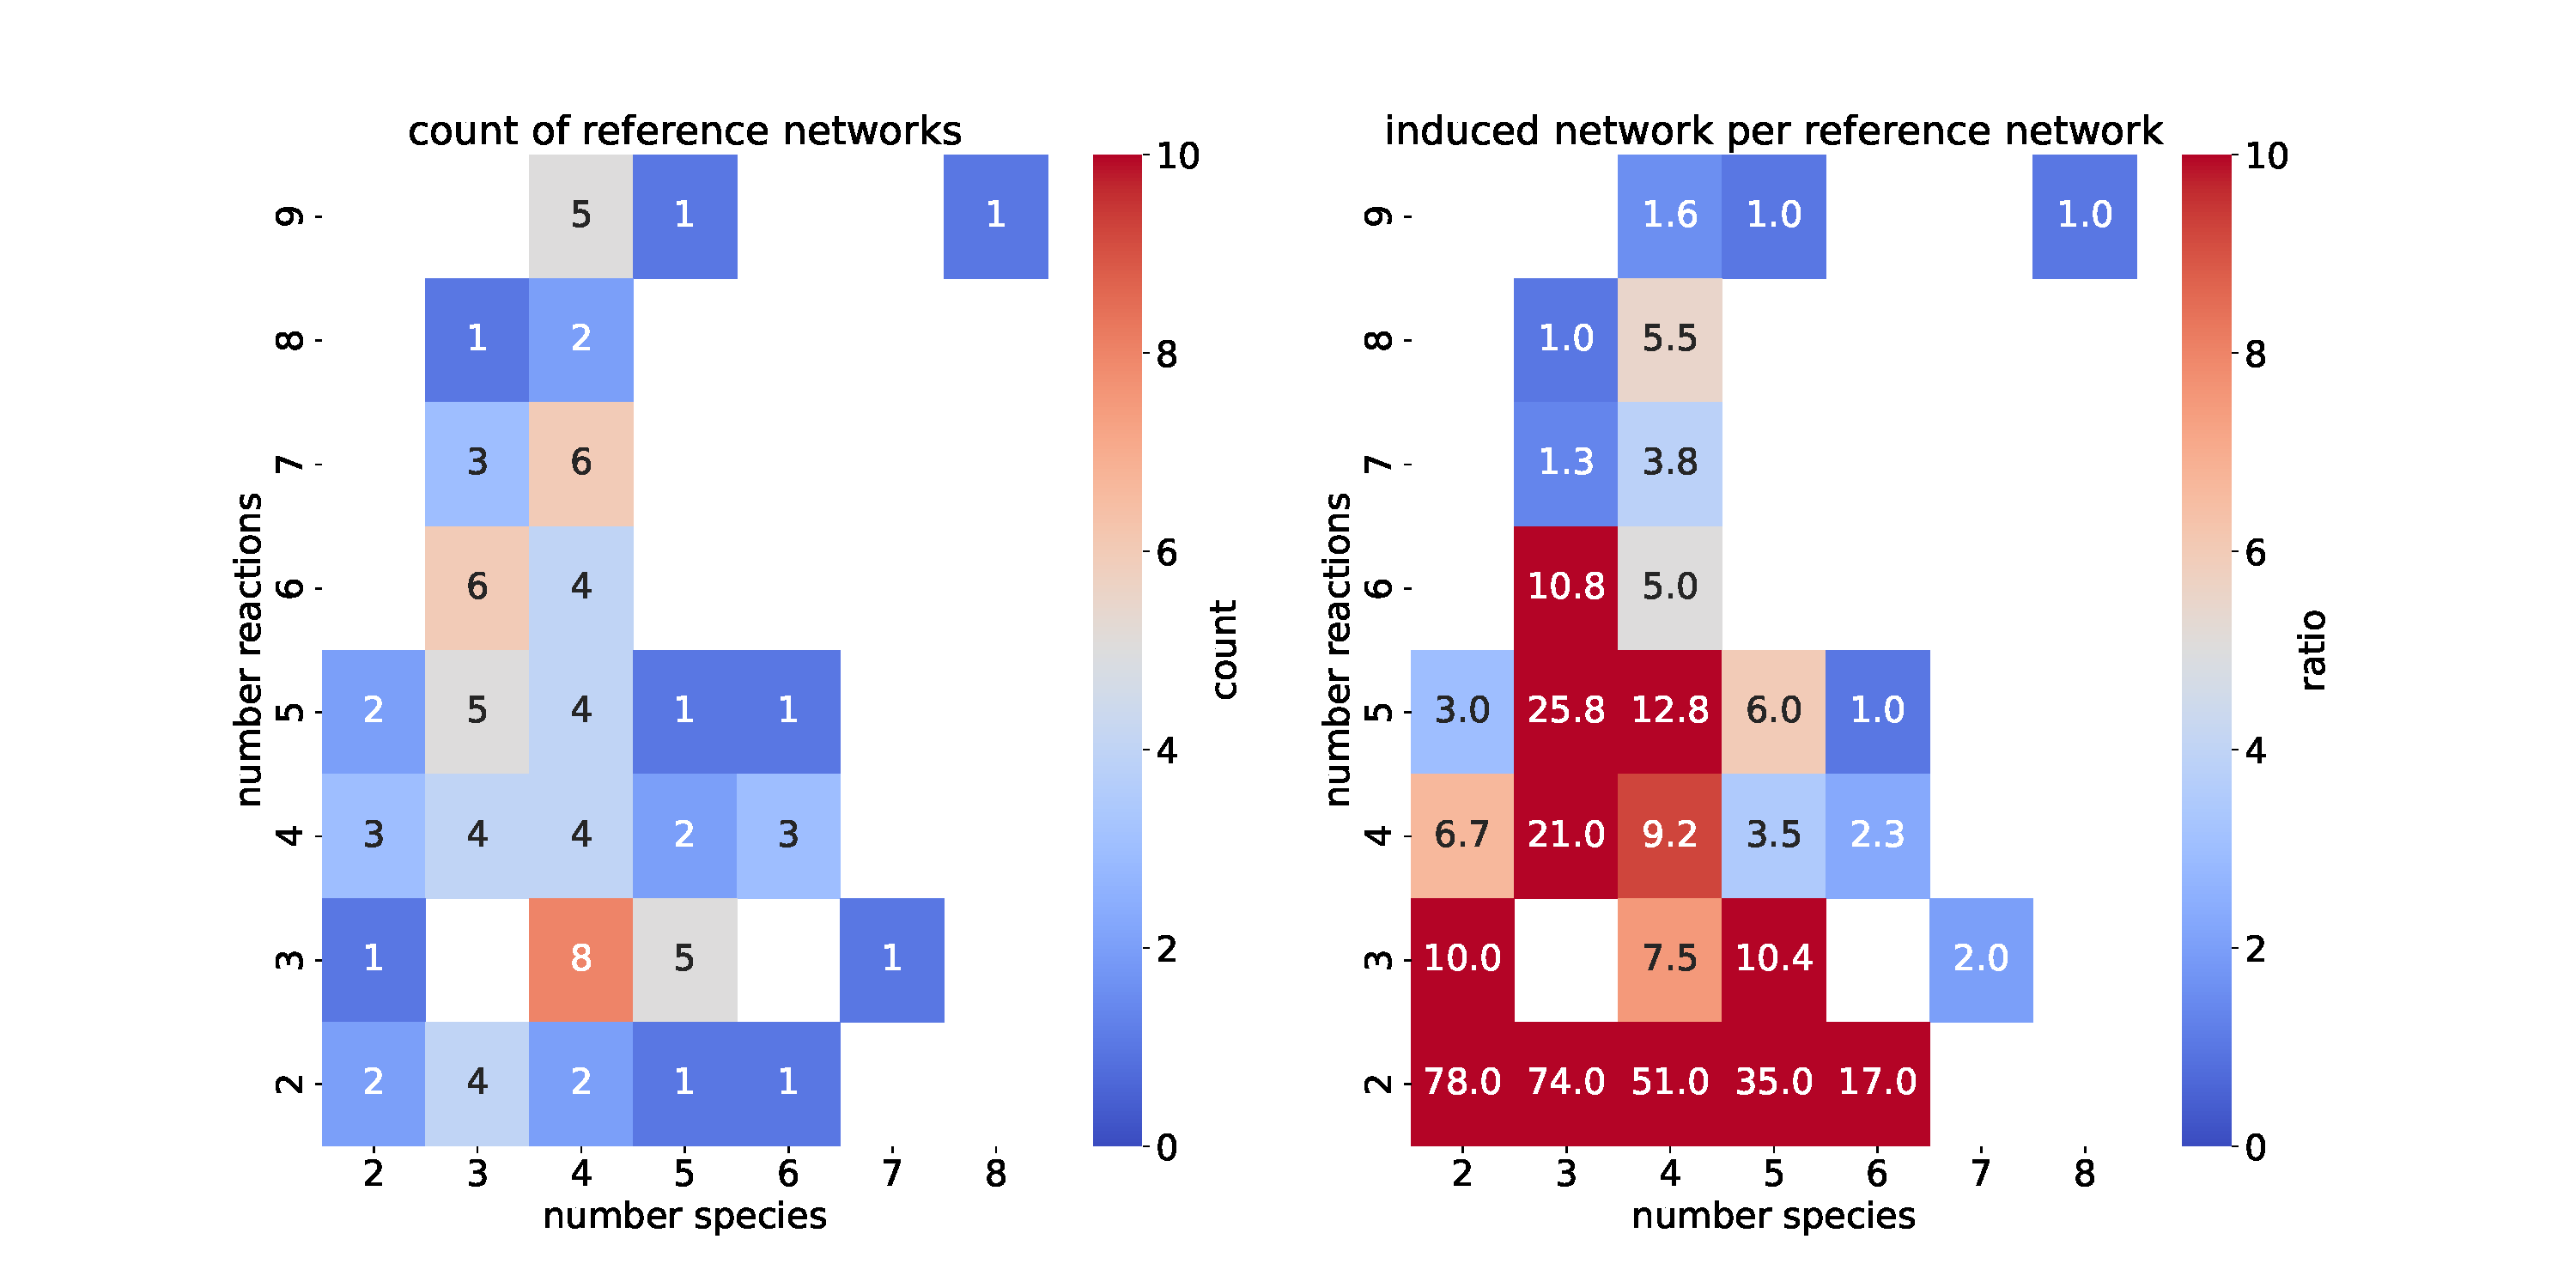
\includegraphics[width=0.5\textwidth, angle=0]{figures/biomodels_results.pdf}
%\caption{Summary of subnet discovery for strong identity for BioModels. The left heatmap displays the sizes of the reference that produced induced networks. The right plot indicates the number of induced networks discovered for reference networks of different sizes.}
%\label{fig:biomodels}
%\end{figure}
%%%%%

%%%%%
%%\begin{figure}
%{\tiny 
%\begin{verbatim}
%%pRB_phosphorylation:  pRB -> pRBp
%pRBp_phosphorylation:  pRBp -> pRBpp
%pRBpp_dephosphorylation:  pRBpp -> pRBp
%pRBp_dephosphorylation:  pRBp -> pRB
%\end{verbatim}
%}
%\caption{BioModels 27}\label{fig:model27}
%\end{figure}
%%%%%

%%%%%
%\begin{figure}
%\hspace{0.2in}
%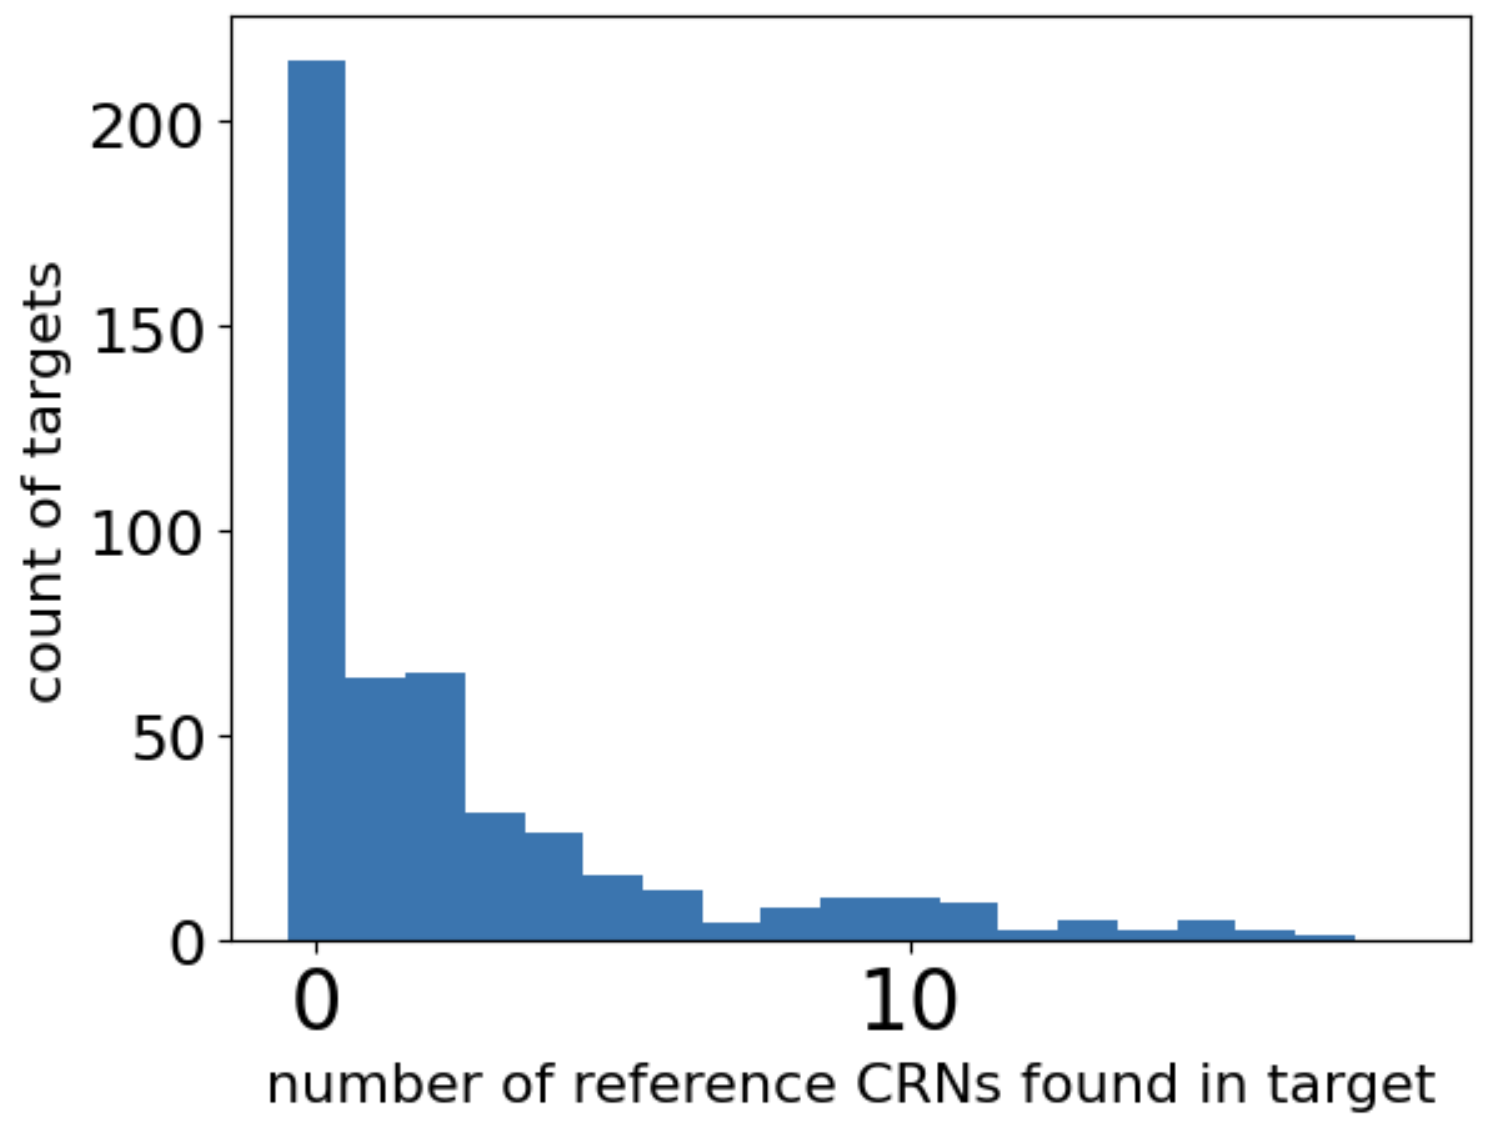
\includegraphics[width=0.2\textwidth, angle=0]{figures/histogram-embedded-subnets.png}
%\caption{Larger models frequently contain one or more smaller models. Approximately half of the 489 target models (>10 reactions, species) contain at least one subnet from a reference model.}
%\label{fig:embedded-models}
%\end{figure}
%%%%%

This section studies the occurrence of subnets \revision{in
the curated branch of BioModels, approximately 1,000 models.
(See \texttt{data/README.md} in the \texttt{github} repository
for details.)}
Reference CRNs are models with no more than 10 reactions;
target models have more than 10 reactions.
To manage computational demands, \revision{we set the API parameter \texttt{max\_num\_mapping\_pair} so that we evaluate at most
$10^{12}$ mapping pairs for a subnet discovery.}
Both weak and strong identity are considered.
\fig{fig:biomodels-summary} summarizes our studies for approximately 200,000 reference-target pairs.
The elapsed time for the studies was slightly less than 14 h on a 128 GB, 20 core Mac Studio M1.
%The full results of our analysis of BioModels are contained in comma separated variable (CSV) files in
%\url{https://github.com/ModelEngineering/pySubnetSB/tree/main/data}.
%The structure of these files is described in the \texttt{README} file in the folder.

%\fig{fig:biomodels} summarizes the results for strong identity; the results for weak identity are similar. The heatmap on the left displays the sizes of the reference CRNs that produced induced networks in the target models. The heatmap on the right displays the number of induced networks discovered per reference CRN. Note that smaller reference CRNs tend to be induced more frequently, which is consistent with our discussion of statistical significance in \secref{sec:significance}.

%\fig{fig:embedded-models} displays a histogram of the number of reference models found in target models. Over half of the targets have at least one reference model as a subnet, and many target models contain five or more reference models. This situation suggests that BioModels could be organized in a more modular way. For example, the modularization capabilities in the Antimony modeling language \citep{smith_antimony_2009} provide a way to structure large models as a combination of smaller models. In so doing, the interrelationships between the models would be more apparent, and revisions to the smaller models could readily be incorporated into the larger models.

%%%%%%%%%%%%
\revision{
\subsection{Use Case 1: Inferring Function in Targets}
}
Here we consider Use Case 1 in the introduction, that the presence of the reference CRN in the target suggests
that functions of the reference are in the target.
The reference CRN is Model 10, which studies ultrasensitivity and negative feedback  in a mitogen-activated protein kinase (MAPK) cascade.
The model has 10 reactions and 7 species.
It turns out that this reference CRN is a subnet of several target models: (i) Model 146 (34 reactions), which investigates MAPK and Akt pathways in heregulin-induced ErbB signaling; (ii) Model 270 (42 reactions), which analyzes isoform-specific ERK signaling and cell fate decisions; and (iii-iv) Models 466 (28 reactions) and 468 (74 reactions), which study shear-stress-induced nitric oxide production in endothelial cells.
\revision{We have strong confirmation that the MAPK function is present in the targets
since the paper associated with each model explicitly states that MAPK function is part of their model.}

\revision{We present another example of Use Case 1.
This
example lacks the strong
confirmation provided in the first example,
but it illustrate how subnet discovery can be used
to generate interesting hypotheses.
We} ask the question ``Are there models in BioModels that contain hidden oscillators?"
We are aided in pursuing this question by the existence of a substantial database
of generated oscillatory CRNs constructed as described in \citep{tatka_cesium_2023}.
We used 6,000 of these generated models as reference CRNs and all of BioModels as target CRNs
to do subnet discovery with weak identity.
It turns out that one of the reference models, the oscillator in \fig{fig:generated-oscillator}, is a statistically significant subnet of three models in BioModels: (i) Model 480 (mucosal immune responses during {\em Helicobacter pylori} infection), (ii) Model 695 (effect of blue light irradiation on reducing the severity of psoriasis vulgaris), and (iii) Model 872 (HIV-associated immunosuppression on HPV persistence in the oral mucosa).
The published papers for the targets make no reference to oscillatory characteristics in these models.
%Although the presence of \fig{fig:generated-oscillator} in multiple targets is an interesting finding, it is beyond the scope of this paper to determine if there is a research result from this finding.

%One interesting finding relates to Model 519. Phosphorylation cycles are common in biology. For example, BioModels 27 is a double phosphorylation cycle consisting of four reactions in \fig{fig:model27}. To our surprise, we discovered only four target models with subnets that are structurally equivalent to the foregoing: 170 (circadian oscillator), 228 (regulatory modules of the mammalian G1/S transition), 354 (calcium signaling), and 355 (an adaptive version of 354). On the other hand, the same model structure appears in surprising places. This model, which is shown in \fig{fig:compare-models}(a), addresses the transformation of stem cells in the colon crypt in the early stages of colorectal cancer. It has 7 reactions and 3 species, which is statistically significant at the level $10^{-5}$ in \fig{fig:statistical-significance}. Model 519 is a weakly identical subnet of six targets: 290 (T-cell regulation),  539 (a theoretical mixed gene model), 687 (cytomegalovirus infection model with cytotoxic T lymphocyte response),848 (immune response to hepatitis B), 852 (chronic inflammation in the development and progression of myeloproliferative neoplasms) and Model 1059 (regulation of caspase-3 activation and degradation in apoptosis). Since four of the six targets have a direct relationship with the immune system (and Model 1059 may have an indirect connection through T-cell-induced apoptosis), these findings motivate an investigation into potential relationships between the mechanisms in early stage cancer and the mechanisms in immune response. We note that in the published papers for these models, none of the six target models reference 519 or overlap with the authors of Model 519.

\revision{
\subsection{Use Case 2: Inferring Common Mechanisms}
}
A common mechanism seems plausible if: (a) there are multiple targets that
have an inferred network for the same reference; and (b) there is
plausible explanation for why the targets might embed the same reference CRN.
A potential common mechanism in our studies is
Model 1059, which addresses the regulation of caspase-3 activation and degradation in apoptosis and has 7 reactions and three species.
The target models in BioModels that have an inferred subnet for 1059 are: Model 156 (oscillations and variability in the p53 system); Model 546 (early immune response and adaptive immune response kinetics in mice infected with influenza A virus); Model 789 (interaction between cancer cells and an oncolytic virus); Model 1012 (cell therapy in B-cell acute lymphoblastic leukemia); and Model 1048 (designing a cancer therapy).
We note that all targets are related to intracellular immune response and/or cell death,
and apoptosis is key to these processes.
\revision{This gives us an interesting hypothesis about a common mechanism.}
%although further work is required to determine if there is a research result.


%%%%%
\begin{figure}
\centering
%\begin{minipage}{1.2in}
%{\tiny
%\begin{verbatim}
%R0X: N0  ->
%R01: N0 -> N0 + N1
%R00: N0 -> 2.0 N0
%R1X: N1 ->
%R12: N1 -> N1 + N2
%R11: N1 -> 2.0 N1
%R2X: N2  ->
%\end{verbatim}
%}
%{\bf {\tiny (a) Model 519}}
%\end{minipage}
%%%
%\begin{minipage}{1.2in}
{\tiny
\begin{verbatim}
J1: S3 -> S2
J2: S0 -> S4 + S0
J3: S4 + S2 -> S4
J4: S2 -> S0 + S2
J5: S4 + S0 -> S4
J6: S2 -> S2 + S2
J7: S2 + S4 -> S2
\end{verbatim}
}
%{\bf {\tiny (b) oscillator}}
%\end{minipage}
\caption{An oscillating CRN that is a subnet of several models in BioModels.}\label{fig:generated-oscillator}
\end{figure}
%%%%%

%\subsection{Subnet Discovery in Practice}
%\begin{enumerate}
%    \item Managing `texttt{max\_num\_mapping\_pair}
%    \item Detecting and resolving large memory consumption.
%\end{enumerate}

%Our study of subnet discovery in BioModels analyzed over 200,000 reference-target pairs. Considerable speedup is possible if these pairs are processed in parallel.

%It turns out that is quite challenging to realize these speedups. For $N$ cores, we achieve a speedup of $N$ relative to a single core if we assign an equal amount of work to each core. An approach is to assign approximately the same number of reference-target pairs to each core. But some reference-target pairs are processed in milliseconds (e.g. if constraints are violated). Other pairs can take several hours (if there are a large number of species/reaction mappings). The result is that assigning an equal number of pairs to cores causes a few cores to have orders of magnitude more work than other cores. So, speedup is limited.

%One solution to the above is to dynamically assign reference-target pairs to processing cores. Unfortunately, Python multiprocessing is very inefficient for such schemes. Instead, we adopted a two-phase approach that better balances work on cores. First, we process all reference-target pairs that require very little computation by using a relatively small value for the maximum number of species/reaction mappings for the pair (1,000). The vast majority of pairs can be processed in this way. In particular, \py{} constraints are quite computationally efficient in detecting the {\em absence} of a subnet (see \fig{fig:scalable-subnet-discovery}), and from \fig{fig:biomodels-summary} fewer than 1.5\% of target pairs have an induced subnet. Thus, the first phase processes reference-target pairs as follows: (a) pairs are processed in parallel;  the maximum number of species/reaction mappings is low (1,000); and species/reaction mappings for a reference-target pair are processed sequentially. The second phase processes pairs with high computational requirements as follows: (a) pairs are processed sequentially;(b) the maximum number of species/reaction mappings is large ($10^{12}$); and (c) species/reaction mappings are processed in parallel. All processes consistently had utilizations in excess of 90\%, an indication that productive computational work is being done.

%%%%%%%%%%%%%%%%%%%%%
\section{Conclusions and Future Work}
Subnet discovery is a powerful tool for generating hypotheses related to the presence of function and conserved mechanisms in CRNs.
%For chemical reaction networks (CRNs), this means finding a subset of reactions in a target CRN that are a simple renaming of the reactions and species in a reference network.
Subnet discovery is a kind of subgraph problem, and these problems are extremely demanding computationally.

This article introduces \py{}, an open source Python package that discovers subnets in CRNs represented using the SBML community standard.
\py{} employs a constraint-based approach that  greatly reduces computations.
\revision{In our studies of randomly selected target networks with
100 reactions that each embed a distinct reference networks with 20 reactions, the number of mapping pairs is reduced from
a computationally infeasible $10^{78}$ to a more practical $10^{8}$.}
\py{} employs a constraint-based approach that  greatly reduces computations (e.g. in our studies, from  the evaluation of an infeasible $10^{78}$ mapping pairs to a more practical $10^{8}$ mapping pairs).
Furthermore, our implementation provides large speedups as a result of vectorization and process-based parallelism
(e.g. a speedup of 400 in our studies).
In addition, we develop a methodology that assesses the statistical significance of subnet discovery.
Last, we use \py{} to study subnets in BioModels
for approximately 200,000 pairs of reference and target models.
We show that for a reference MAPK pathway, subnet discovery correctly indicates the presence of MAPK function in several target models.
The studies also suggest a couple of interesting hypotheses: (a) the presence of hidden oscillators in several models in BioModels,
and (b) a conserved mechanism for intracellular immune response.

In the near term, we want to increase the computational speed of \py{} by making use of Graphics Processing Units (GPUs).
\revision{Longer term, we plan to explore the hypotheses identified in our discovery of subnets in BioModels.}

%%%%%%%%%%%%%%%%%%%%%%%%%%
\section*{Author Contributions}
JLH (problem formulation and approach; implementation; BioModels studies; first draft),
LPS (co-developed subnet identity; co-designed generation of random CRNs; oscillator discovery),
LTT (oscillator discovery),
SSA (critical early stage feedback),
MAK (oscillator data), 
HMS (critical early stage feedback; oscillator discovery).

%%%%%%%%%%%%%%%%%%%%%%%
\section*{Acknowledgements}
\revision{Our deep appreciation to the reviewers for their thoughtful comments.}
We acknowledge support from the eScience Institute at the University of Washington, and NIBIB of the National Institutes of Health under grant number NIH P41EB023912.
% Reviewers: \item Anatasia, Rahuman, Uri Alon, Matthias

\bibliographystyle{natbib}
\bibliography{refs}

\end{document}
